\documentclass[11pt]{article}

\usepackage[margin=1in]{geometry}
\usepackage{amsmath,amssymb,amsthm}
\usepackage{booktabs}
\usepackage[authoryear,round]{natbib}
\usepackage{graphicx}
\usepackage{placeins}
\usepackage{float}
\usepackage{caption}
\captionsetup[figure]{name=Fig., labelsep=space, labelfont=bf}
\usepackage[hidelinks,pdfauthor={Diogo Ribeiro},pdftitle={Sparse Contamination in Tail-Index Estimation: Detectability, Negligibility, and Risk}]{hyperref}
\setlength{\emergencystretch}{2em}

% The reporting tables in Section 12 are tall; without these the whole set
% floats past its own discussion to the end of the document.
\renewcommand{\topfraction}{0.9}
\renewcommand{\bottomfraction}{0.8}
\renewcommand{\textfraction}{0.07}
\renewcommand{\floatpagefraction}{0.75}
\setcounter{topnumber}{3}
\setcounter{totalnumber}{4}

\newtheorem{theorem}{Theorem}
\newtheorem{proposition}{Proposition}
\newtheorem{lemma}{Lemma}
\newtheorem{corollary}{Corollary}
\newtheorem{remark}{Remark}

\DeclareMathOperator{\Var}{Var}
\DeclareMathOperator{\E}{E}
\newcommand{\Pp}{\mathbb{P}}
\newcommand{\ghat}{\widehat{\gamma}}

\title{Sparse Contamination in Tail-Index Estimation:\\
Detectability, Negligibility, and Risk}
\author{%
Diogo Ribeiro\\[4pt]
\normalsize Faculty of Media Arts and Design, Technical University of Porto,\\
\normalsize Porto, Portugal\\[2pt]
\normalsize ORCID \texttt{0009-0001-2022-7072}\\[2pt]
\normalsize Corresponding author: \texttt{dfr@esmad.ipp.pt}%
}
\date{30 August 2026}

\begin{document}
\maketitle

\begin{abstract}
Robust tail-index estimators are usually judged by whether they identify the
contaminated extremes.  This paper separates that diagnostic target from two
decision targets: mean-squared-error (MSE) worthwhile intervention and
first-order risk relevance.
In an exact Pareto model, multiplying the largest $r_n$ observations by
$\Delta_n$ shifts exactly one normalized log-spacing, by
$S_n=r_n\log\Delta_n$.  Three thresholds in $S_n$ govern three questions.
Trimmed-Hill oracle intervention repays its variance cost above
$\gamma\{r_nk_n/(k_n-r_n)\}^{1/2}$; the conservative
spacing scan detects the contaminated boundary above $\gamma\log(h_n/\alpha_n)$
for scan size $h_n$ and level $\alpha_n$; and ordinary
Hill risk is disturbed at first order only at $\gamma\sqrt{k_n}$.  For bounded
contamination counts these are ordered
\[
  \gamma\sqrt{r_nk_n/(k_n-r_n)}
  \ll
  \gamma\log(h_n/\alpha_n)
  \ll
  \gamma\sqrt{k_n},
\]
so the three are distinct.  The main first-order result is a
detect-or-ignore theorem: strong contamination is detected and removed, while
weak contamination can be missed without changing the first-order limit
distribution.  A pre-specified Monte Carlo experiment of 5000 paired
replications reproduces the two exact risk identities and exhibits the
predicted detection transition, and bounded-influence estimators outperform
adaptive trimming in part of the region where intervention is worthwhile but
recovery is unreliable.  Post-specified stress tests bound the detection
scale's scope: contamination spread across several
spacings damages Hill identically while remaining nearly undetectable.  For
ordered unequal factors, Hill damage is governed by the sum of the local
spacing shifts and scan detectability by their largest component, so
localization rather than total magnitude is the relevant diagnostic quantity.
\end{abstract}

\noindent\textbf{Keywords} extreme value theory $\cdot$ tail index $\cdot$
Hill estimator $\cdot$ robust estimation $\cdot$ adaptive trimming $\cdot$
sparse contamination

\medskip
\noindent\textbf{Mathematics Subject Classification} 62G32 $\cdot$ 62G35
$\cdot$ 62G20

\section{Question}

Recovering the contaminated observations and controlling squared-error risk are
different objectives, and it is not obvious that the first is needed for the
second:
\[
  \hbox{does a robust estimator need to recover every contaminated extreme}
  \quad
  \hbox{to have good risk?}
\]
The analysis below shows that the answer is no, at least in the structured
exact-Pareto contamination model studied here.  Exact recovery is a diagnostic
target.  Squared-error
risk is a decision target.  Sparse contamination can be worth removing for an
oracle, too weak for a conservative detector to recover reliably, and still too
weak to matter at the ordinary first-order sampling-error scale.

The model is deliberately structured extremal contamination: the top $r_n$
clean order statistics are modified after their ranks are known.  This is a
stress-test model for tail robustness, not generic Huber contamination and not
randomly placed measurement error.

The key signal in the equal-strength model is
\[
  S_n=r_n\log\Delta_n,
\]
where $r_n$ is the number of top observations perturbed and $\Delta_n$ is their
multiplicative strength.  The same signal appears in the exact MSE gain from
oracle trimming, in spacing-test detectability and in Hill bias.  The point of
the paper is that those appearances use different normalizing scales.

\section{Exact Pareto Spacing Model}

Let $X_1,\ldots,X_n$ be exact Pareto with survival function
\[
  \overline F(x)=x^{-1/\gamma},\qquad x\ge1,\quad \gamma>0.
\]
Write the descending order statistics as
\[
  X_{1:n}\ge X_{2:n}\ge\cdots\ge X_{n:n}.
\]
For $j=1,\ldots,k_n$, define the normalized upper log-spacings
\[
  Z_j=j\{\log X_{j:n}-\log X_{j+1:n}\}.
\]
By the exponential spacing representation \citep{renyi-1953},
$Z_1,\ldots,Z_{k_n}$ are independent exponential random variables with mean
$\gamma$.  This exactness is specific to the Pareto model, but the
log-spacing representation itself is not: for Pareto-type tails the same
spacings admit an approximate exponential representation with a second-order
remainder \citep{beirlant-dierckx-guillou-starica-2002}, which is the sense in
which the calculations below are a controlled benchmark rather than an
isolated special case.

The ordinary Hill estimator at threshold $k_n$ is
\[
  \ghat_H(k_n)=\frac1{k_n}\sum_{j=1}^{k_n}Z_j.
\]
The fixed-$r$ trimmed Hill estimator is
\[
  \ghat_T(r,k_n)=\frac1{k_n-r}\sum_{j=r+1}^{k_n}Z_j.
\]

\section{Sparse Multiplicative Contamination}

For integers $0\le r_n<k_n$, define the contaminated ordered sample by
\[
  X^\star_{j:n}
  =
  \begin{cases}
    \Delta_n X_{j:n}, & 1\le j\le r_n,\\
    X_{j:n}, & j>r_n,
  \end{cases}
  \qquad \Delta_n\ge1.
\]
Multiplying the top $r_n$ clean order statistics by the same factor preserves
their internal log-gaps.  It changes only the boundary gap below the last
perturbed observation.

\begin{lemma}[Boundary-spacing identity]
\label{lem:boundary}
Let
\[
  Z^\star_j
  =
  j\{\log X^\star_{j:n}-\log X^\star_{j+1:n}\}.
\]
If $r_n\ge1$, then
\[
  Z^\star_j=Z_j\quad(j\ne r_n),
  \qquad
  Z^\star_{r_n}=Z_{r_n}+r_n\log\Delta_n.
\]
Consequently,
\[
  \ghat^\star_H(k_n)-\ghat_H(k_n)
  =
  \frac{S_n}{k_n},
  \qquad
  S_n=r_n\log\Delta_n.
\]
\end{lemma}

\begin{proof}
For $j<r_n$, both $X_{j:n}$ and $X_{j+1:n}$ are multiplied by $\Delta_n$, so the
log-ratio is unchanged.  For $j>r_n$, neither value is multiplied.  At
$j=r_n$, only the upper value is multiplied, so the log-ratio increases by
\[
  \log(\Delta_n X_{r_n:n})-\log X_{r_n+1:n}
  -
  \{\log X_{r_n:n}-\log X_{r_n+1:n}\}
  =
  \log\Delta_n.
\]
Multiplication by the spacing index $r_n$ gives the displayed identity.  The
Hill identity follows by averaging the first $k_n$ normalized spacings.
\end{proof}

\begin{remark}
If $r_n=0$, then $S_n=0$ and the identities are read with no contaminated
boundary.  The equal-factor model is the cleanest version of the
sparse-contamination question because detection and Hill bias collapse to one
scalar signal.
\end{remark}

\begin{lemma}[Unequal multiplicative factors]
\label{lem:unequal}
Let the top $r$ clean order statistics be multiplied by positive factors
\[
  \Delta_1\ge\Delta_2\ge\cdots\ge\Delta_r\ge1,
  \qquad
  \Delta_{r+1}=1,
\]
so that their order is preserved.  Then, for $j\le r$,
\[
  Z_j^\star
  =
  Z_j+j\log\frac{\Delta_j}{\Delta_{j+1}},
\]
and $Z_j^\star=Z_j$ for $j>r$.  Consequently,
\[
  \ghat_H^\star(k)-\ghat_H(k)
  =
  \frac1k\sum_{j=1}^{r}\log\Delta_j .
\]
\end{lemma}

\begin{proof}
For $j\le r$, subtracting the contaminated and clean log-gaps gives
\[
  \{\log(\Delta_jX_{j:n})-\log(\Delta_{j+1}X_{j+1:n})\}
  -
  \{\log X_{j:n}-\log X_{j+1:n}\}
  =
  \log(\Delta_j/\Delta_{j+1}).
\]
Multiplication by $j$ gives the spacing identity.  The Hill shift is
\[
  \frac1k\sum_{j=1}^{r}j\log(\Delta_j/\Delta_{j+1})
  =
  \frac1k\sum_{j=1}^{r}\log\Delta_j,
\]
by summation by parts, using $\Delta_{r+1}=1$.
\end{proof}

\begin{remark}
Outside the equal-factor model, detection and Hill risk do not depend on the
same scalar.  Detection responds to local spacing jumps
$j\log(\Delta_j/\Delta_{j+1})$, while Hill bias responds to the cumulative
sum $\sum_{j=1}^r\log\Delta_j$.
\end{remark}

\begin{remark}
\label{rem:delta}
Collect those jumps into a vector.  Write
\[
  \delta_j
  =
  Z_j^\star-Z_j
  =
  j\log\frac{\Delta_j}{\Delta_{j+1}},
  \qquad j=1,\ldots,r,
\]
with $\Delta_{r+1}=1$, and $\boldsymbol\delta=(\delta_1,\ldots,\delta_r)$.
The ordering $\Delta_1\ge\cdots\ge\Delta_r\ge1$ makes $\delta_j\ge0$, and the
summation by parts in the proof of Lemma \ref{lem:unequal} says exactly that
\[
  \sum_{j=1}^r\delta_j=\sum_{j=1}^r\log\Delta_j,
\]
so the Hill shift is the $\ell^1$ norm of the shift vector,
\[
  \ghat_H^\star(k)-\ghat_H(k)
  =
  \frac{\|\boldsymbol\delta\|_1}{k}.
\]
In the equal-factor case only the boundary spacing moves,
$\boldsymbol\delta=(0,\ldots,0,S)$ with $S=r\log\Delta$, so
$\|\boldsymbol\delta\|_1=S$ and the scalar notation used throughout the rest
of the paper is recovered.
\end{remark}

\section{Detection Scale}
\label{sec:detection-scale}

The adaptive trimming rule in the \texttt{heavytails} package tests
normalized spacings against
the mean of deeper spacings.  For a candidate boundary $j$, write
\[
  R_j=\frac{Z_j}{\overline Z_{j+1:k_n}},
  \qquad
  \overline Z_{j+1:k_n}=\frac1{k_n-j}\sum_{\ell=j+1}^{k_n}Z_\ell.
\]
Under the exact Pareto null,
\[
  \Pp_0(R_j>t)
  =
  \left(\frac{m}{m+t}\right)^m,
  \qquad m=k_n-j.
\]
Testing $h_n$ possible trim boundaries at family-wise level $\alpha_n$ gives
the Bonferroni pointwise level
\[
  a_n=\alpha_n/h_n.
\]
The rejection threshold is therefore
\[
  t_{m,a_n}
  =
  m\{a_n^{-1/m}-1\}.
\]
If $\log(1/a_n)=o(m)$, then
\[
  t_{m,a_n}
  =
  \log(1/a_n)\{1+o(1)\}
  =
  \log(h_n/\alpha_n)\{1+o(1)\}.
\]

\begin{proposition}[Boundary detectability]
\label{prop:detectability}
Assume $1\le r_n\le h_n<k_n$, $m_n=k_n-r_n\to\infty$,
$\alpha_n\to0$ and $\log(h_n/\alpha_n)=o(m_n)$.  Let
\[
  L_n=\log(h_n/\alpha_n).
\]
Under the sparse contamination model of Lemma \ref{lem:boundary}, the boundary
test at $j=r_n$ satisfies:
\[
  \frac{S_n}{\gamma L_n}\ge 1+\varepsilon
  \quad\Longrightarrow\quad
  \Pp(\hbox{boundary detected})\to1,
\]
and
\[
  \frac{S_n}{\gamma L_n}\le 1-\varepsilon
  \quad\Longrightarrow\quad
  \Pp(\hbox{boundary detected})\to0,
\]
for every fixed $\varepsilon>0$.
\end{proposition}

\begin{proof}
At the contaminated boundary,
\[
  R^\star_{r_n}
  =
  \frac{Z_{r_n}+S_n}{\overline Z_{r_n+1:k_n}}.
\]
The denominator converges in probability to $\gamma$ by the law of large
numbers, since $m_n\to\infty$.  Also $Z_{r_n}=O_p(1)$, while
$L_n\to\infty$.  Hence
\[
  \frac{R^\star_{r_n}}{L_n}
  =
  \frac{S_n}{\gamma L_n}+o_p(1).
\]
The exact rejection threshold obeys $t_{m_n,a_n}/L_n\to1$.  The two claims
follow by comparison with this threshold.
\end{proof}

\begin{theorem}[Exact recovery by deepest-first scan]
\label{thm:exact-recovery}
In the equal-factor contamination model, define the deepest-first scan by
\[
  \widehat r_n
  =
  \max\{j\le h_n:p_j\le\alpha_n/h_n\},
\]
with $\widehat r_n=0$ if the set is empty, where $p_j$ is the exact spacing
p-value.  Assume $1\le r_n\le h_n<k_n$, $k_n-r_n\to\infty$,
$\alpha_n\to0$, $\log(h_n/\alpha_n)=o(k_n-r_n)$ and, for some
$\varepsilon>0$,
\[
  S_n\ge(1+\varepsilon)\gamma\log(h_n/\alpha_n).
\]
Then
\[
  \Pp(\widehat r_n=r_n)\to1.
\]
\end{theorem}

\begin{proof}
By Proposition \ref{prop:detectability}, the contaminated boundary $j=r_n$ is
rejected with probability tending to one.  If no deeper clean spacing
$j>r_n$ is falsely rejected, the maximum rejected index is therefore exactly
$r_n$.  For every $j>r_n$, the spacing and all deeper spacings are unchanged
exact-Pareto spacings, so the corresponding null p-value is uniform.  A union
bound gives
\[
  \Pp\{\exists j>r_n:p_j\le\alpha_n/h_n\}
  \le
  (h_n-r_n)\frac{\alpha_n}{h_n}
  \le
  \alpha_n
  \to0.
\]
Combining boundary detection with the vanishing probability of a deeper false
rejection proves the result.
\end{proof}

Exact recovery has the same leading boundary as detecting the contaminated
boundary, provided the boundary is inside the scan and the equal-factor model
holds.  This is stronger than detecting some anomaly, but it is still a
detection statement rather than a risk statement.

\section{First-Order Hill Risk Scale}

Under the clean exact Pareto model,
\[
  \sqrt{k_n}\{\ghat_H(k_n)-\gamma\}
  \Rightarrow
  N(0,\gamma^2).
\]
Lemma \ref{lem:boundary} gives the contaminated estimator
\[
  \sqrt{k_n}\{\ghat^\star_H(k_n)-\gamma\}
  =
  \sqrt{k_n}\{\ghat_H(k_n)-\gamma\}
  +
  \frac{S_n}{\sqrt{k_n}}.
\]
Therefore the contamination is negligible on the ordinary sampling-error scale
when
\[
  S_n=o(\gamma\sqrt{k_n}),
\]
and first-order relevant when
\[
  S_n\asymp\gamma\sqrt{k_n}.
\]
It dominates ordinary sampling error when
\[
  S_n/(\gamma\sqrt{k_n})\to\infty.
\]

\begin{proposition}[Hill risk shift]
\label{prop:risk}
For fixed $k_n$ under exact Pareto sampling and the contamination model above,
\[
  \E\{\ghat^\star_H(k_n)-\gamma\}=\frac{S_n}{k_n},
  \qquad
  \Var\{\ghat^\star_H(k_n)\}=\frac{\gamma^2}{k_n}.
\]
Thus
\[
  \operatorname{MSE}\{\ghat^\star_H(k_n)\}
  =
  \frac{\gamma^2}{k_n}
  +
  \frac{S_n^2}{k_n^2}.
\]
\end{proposition}

\begin{proof}
The contaminated estimator is the clean Hill estimator plus the deterministic
shift $S_n/k_n$.  The clean Hill estimator is unbiased with variance
$\gamma^2/k_n$ because it averages $k_n$ independent exponential spacings with
mean $\gamma$ and variance $\gamma^2$.
\end{proof}

\section{Trimmed-Hill Intervention Scale}
\label{sec:oracle-scale}

The $\sqrt{k_n}$ scale is a first-order scale.  It is not the exact threshold
at which robustification begins to improve MSE.  If an oracle knows the true
contamination count $r_n$, it can remove the shifted boundary spacing entirely
by using $\ghat_T(r_n,k_n)$.

\begin{proposition}[Oracle trimming intervention threshold]
\label{prop:oracle-intervention}
Under the equal-factor contamination model with $0<r<k$, the oracle trimmed
Hill estimator satisfies
\[
  \operatorname{MSE}\{\ghat_T(r,k)\}
  =
  \frac{\gamma^2}{k-r}.
\]
Compared with the contaminated Hill estimator,
\[
  \operatorname{MSE}\{\ghat_T(r,k)\}
  -
  \operatorname{MSE}\{\ghat_H^\star(k)\}
  =
  \frac{\gamma^2r}{k(k-r)}
  -
  \frac{S^2}{k^2},
\]
where $S=r\log\Delta$.  Therefore oracle trimming improves exact MSE if and
only if
\[
  S^2>\gamma^2\frac{rk}{k-r}.
\]
The exact-MSE intervention threshold is
\[
  I^{T}_{r,k}
  =
  \gamma\sqrt{\frac{rk}{k-r}},
\]
and, if $r=o(k)$,
\[
  I^{T}_{r,k}\sim\gamma\sqrt r.
\]
\end{proposition}

\begin{proof}
After trimming the first $r$ spacings, the shifted boundary spacing
$Z_r^\star$ is absent.  The remaining $k-r$ spacings are unchanged independent
exponentials with mean $\gamma$ and variance $\gamma^2$.  Hence the oracle
trimmed estimator is unbiased and has variance $\gamma^2/(k-r)$.  Proposition
\ref{prop:risk} gives the contaminated Hill MSE.  Subtracting the two MSEs
gives
\[
  \frac{\gamma^2}{k-r}
  -
  \left(
    \frac{\gamma^2}{k}
    +
    \frac{S^2}{k^2}
  \right)
  =
  \frac{\gamma^2r}{k(k-r)}
  -
  \frac{S^2}{k^2}.
\]
The displayed intervention condition and threshold follow by rearrangement.
\end{proof}

\begin{remark}
Any nonzero $S$ changes the exact contaminated-Hill MSE.  Proposition
\ref{prop:oracle-intervention} asks a sharper decision question: when does
oracle robustification compensate for the variance cost of discarding $r$
spacings?
\end{remark}

\begin{remark}
\label{rem:trim-oracle}
The oracle here knows the true trim count within the standard trimmed-Hill
family.  It is not an oracle over arbitrary estimators, and $I^{T}_{r,k}$ is
correspondingly the intervention scale of that family rather than a universal
one.  Under the equal-factor model only the boundary spacing $Z_{r}$ is
shifted, by Lemma \ref{lem:boundary}, so a procedure that knew which spacing
had moved could discard $Z_{r}$ alone and keep $Z_1,\ldots,Z_{r-1}$.  That
estimator has MSE $\gamma^2/(k-1)$, so it improves on contaminated Hill as soon
as
\[
  S^2>\gamma^2\frac{k}{k-1},
  \qquad\hbox{that is}\qquad
  S\gtrsim\gamma,
\]
with no dependence on $r$ at all.  The growth $I^{T}_{r,k}\sim\gamma\sqrt r$
is therefore entirely the price of discarding $r-1$ uncontaminated spacings,
not a property of the contamination: $I^{T}_{r,k}$ measures when a particular
robust action becomes worthwhile, not when intervention as such does.  The
three-scale ordering is unaffected, because both thresholds are $O(1)$ for
fixed $r$.
\end{remark}

\section{Detect or Safely Ignore}

The three-scale picture has a first-order consequence.  An adaptive trimming
rule need not recover every weak contaminated boundary to have the same
first-order behavior as clean Hill.  It is enough that strong contamination is
detected and weak contamination is asymptotically invisible at the
$k_n^{-1/2}$ scale.

\begin{theorem}[Detect-or-ignore first-order robustness]
\label{thm:detect-ignore}
Consider the equal-factor structured contamination model.  Assume
\[
  r_n=O(1),\qquad r_n\le h_n<k_n,\qquad k_n\to\infty,
\]
\[
  \alpha_n\to0,\qquad
  \log(h_n/\alpha_n)=o(k_n-r_n),
\]
and define
\[
  D_n=\gamma\log(h_n/\alpha_n),
  \qquad
  D_n=o(\gamma\sqrt{k_n}).
\]
Let $\widehat r_n$ be the deepest-first scan from Theorem
\ref{thm:exact-recovery}, and define
\[
  \widehat\gamma_A=\widehat\gamma_T(\widehat r_n,k_n).
\]
Then, for every deterministic sequence $\Delta_n\ge1$, equivalently
$S_n=r_n\log\Delta_n\ge0$,
\[
  \sqrt{k_n}(\widehat\gamma_A-\gamma)
  \Rightarrow
  N(0,\gamma^2).
\]
\end{theorem}

\begin{proof}
Let $L_n=\log(h_n/\alpha_n)$, so $D_n=\gamma L_n$.  The proof uses the
subsequence principle.

First take a subsequence along which $S_n>2D_n$ eventually.  Then
$S_n\ge(1+\varepsilon)\gamma L_n$ with $\varepsilon=1$, and Theorem
\ref{thm:exact-recovery} gives $\Pp(\widehat r_n=r_n)\to1$.  On that event,
$\widehat\gamma_A$ is the oracle trimmed estimator.  Since $r_n=O(1)$,
\[
  \Var\{\sqrt{k_n}(\widehat\gamma_T(r_n,k_n)-\gamma)\}
  =
  \frac{k_n\gamma^2}{k_n-r_n}
  \to
  \gamma^2,
\]
and the central limit theorem for the remaining independent exponential
spacings gives the displayed limit.

Now take a subsequence along which $S_n\le2D_n$ eventually.  Because
$D_n=o(\gamma\sqrt{k_n})$,
\[
  \frac{S_n}{\sqrt{k_n}}\to0.
\]
With probability at least $1-\alpha_n+o(1)$, the deepest-first scan does not
trim past the true boundary: the only way to have $\widehat r_n>r_n$ is a false
rejection among clean deeper spacings, whose probability is bounded by
$\alpha_n$ as in Theorem \ref{thm:exact-recovery}.  On the event
$\widehat r_n\le r_n$, the adaptive estimator differs from the clean Hill
estimator by
\[
  \widehat\gamma_A-\widehat\gamma_H
  =
  O_p(k_n^{-1})
  +
  \mathbf 1\{\widehat r_n<r_n\}
  \frac{S_n}{k_n-\widehat r_n}.
\]
The first term is the effect of removing at most $r_n=O(1)$ ordinary
exponential spacings and renormalizing by $k_n-\widehat r_n$ rather than
$k_n$.  The second term is the retained boundary shift when the scan trims too
little.  Since $S_n\le2D_n=o(\gamma\sqrt{k_n})$,
\[
  \sqrt{k_n}(\widehat\gamma_A-\widehat\gamma_H)=o_p(1),
\]
where $\widehat\gamma_H$ is the clean Hill estimator built from the unperturbed
spacings.  The clean Hill central limit theorem gives the same limit.

Every subsequence contains a further subsequence on which either
$S_n>2D_n$ eventually or $S_n\le2D_n$ eventually.  Both further subsequences
converge to the same $N(0,\gamma^2)$ law.  Therefore the full sequence
converges to that law.
\end{proof}

\begin{corollary}[Interlock false refusals vanish inside the scan]
\label{cor:interlock}
Suppose the production deep-contamination interlock scans clean spacings below
the supported trimming envelope at family-wise level
\[
  \delta_n=\min\{10^{-4},n^{-2}\}.
\]
If the true boundary satisfies $r_n\le h_n$, then
\[
  \Pp(\hbox{false interlock refusal})\le\delta_n\to0.
\]
Thus the interlock does not change Theorem \ref{thm:detect-ignore} when the
true contamination boundary lies inside the declared trimming envelope.
\end{corollary}

\begin{proof}
Below the supported trimming envelope the spacings are clean exact-Pareto
spacings under the theorem's model.  Each interlock p-value is uniform under
the null, and the implementation divides the family-wise level across the deep
tests.  A union bound gives the result.
\end{proof}

\begin{corollary}[Missed oracle gains below detection are second-order]
\label{cor:missed-gain}
Let
\[
  G_n
  =
  \operatorname{MSE}\{\widehat\gamma_H^\star(k_n)\}
  -
  \operatorname{MSE}\{\widehat\gamma_T(r_n,k_n)\}.
\]
If $r_n=O(1)$ and
\[
  I^{T}_{r_n,k_n}\ll S_n\ll D_n\ll\gamma\sqrt{k_n},
\]
then oracle trimming improves exact MSE, but
\[
  \frac{G_n}{\gamma^2/k_n}\to0.
\]
\end{corollary}

\begin{proof}
By Proposition \ref{prop:oracle-intervention},
\[
  G_n
  =
  \frac{S_n^2}{k_n^2}
  -
  \frac{\gamma^2r_n}{k_n(k_n-r_n)}.
\]
The assumption $S_n\gg I^{T}_{r_n,k_n}$ makes $G_n>0$ eventually.  Dividing by
$\gamma^2/k_n$ gives
\[
  \frac{G_n}{\gamma^2/k_n}
  =
  \frac{S_n^2}{\gamma^2 k_n}
  -
  \frac{r_n}{k_n-r_n}.
\]
The first term tends to zero because $S_n\ll\gamma\sqrt{k_n}$, and the second
term tends to zero because $r_n=O(1)$ and $k_n\to\infty$.
\end{proof}

\section{Separation}

The preceding propositions give three different scales:
\[
  \hbox{oracle exact-MSE intervention:}
  \qquad
  I^{T}_{r_n,k_n}
  =
  \gamma\sqrt{\frac{r_nk_n}{k_n-r_n}},
\]
\[
  \hbox{detectability:}
  \qquad
  D_n
  =
  \gamma\log(h_n/\alpha_n),
\]
and
\[
  \hbox{first-order Hill-risk relevance:}
  \qquad
  R_n
  =
  \gamma\sqrt{k_n}.
\]

\begin{corollary}[Three-scale separation]
\label{cor:separation}
Suppose $k_n=n^a$ for some $0<a<1$, $r_n=O(1)$,
$h_n\le Ck_n^b$ for fixed $C<\infty$ and $b\ge0$, and
\[
  \alpha_n\asymp(\log n)^{-2}.
\]
Then
\[
  I^{T}_{r_n,k_n}=O(1),
  \qquad
  \log(h_n/\alpha_n)=O(\log n),
  \qquad
  \sqrt{k_n}=n^{a/2},
\]
so
\[
  I^{T}_{r_n,k_n}\ll D_n\ll R_n.
\]
There are asymptotic regions in which
\[
  I^{T}_{r_n,k_n}\ll S_n\ll D_n
  \qquad\hbox{and}\qquad
  D_n\ll S_n\ll R_n.
\]
In the first region oracle trimming improves exact MSE but the conservative
adaptive scan does not reliably recover the boundary.  In the second region
the boundary is detectable but the contamination is negligible at the ordinary
first-order Hill sampling-error scale.
\end{corollary}

The resulting phase diagram is:
\[
\begin{array}{c|c|c|c}
\toprule
\hbox{signal size} &
\hbox{oracle trimming improves MSE?} &
\hbox{detectable?} &
\hbox{first-order risk relevant?}\\
\midrule
S_n\ll I^{T}_{r_n,k_n} & \hbox{no} & \hbox{no} & \hbox{no}\\
I^{T}_{r_n,k_n}\ll S_n\ll D_n & \hbox{yes} & \hbox{no} & \hbox{no}\\
D_n\ll S_n\ll R_n & \hbox{yes} & \hbox{yes} & \hbox{no}\\
S_n\gtrsim R_n & \hbox{yes} & \hbox{yes} & \hbox{yes}\\
\bottomrule
\end{array}
\]

This is the mathematical backbone of this paper.  Exact contamination
recovery is too demanding as a primary objective, and first-order
negligibility is not the same as exact MSE irrelevance.  The decision question
is when contamination is detectable, when it is worth acting on, and when it
alters first-order risk.

\section{Estimator Comparison Implied by the Theory}
\label{sec:estimator-comparison}

The theory calls for comparing two robustness philosophies rather than ranking
estimators.

\paragraph{Detection and removal.}
Adaptive trimmed Hill estimates $r_n$ and removes the first $\widehat r$
normalized spacings.  It is naturally targeted at contamination that is
detectable by the spacing scan; when such contamination also exceeds the
trimmed-Hill intervention scale $I^{T}_{r,k}$, successful recovery can
translate into an MSE benefit.  Its
vulnerability is the intermediate region $I^{T}_{r,k}<S<D_n$: oracle trimming would
improve exact MSE, but the conservative scan may not recover the boundary.  This
belongs to the adaptive
trimming and extreme-outlier detection line of Bhattacharya, Kallitsis and
Stoev \citeyearpar{bhattacharya-kallitsis-stoev-2019}; the point here is not to
replace that estimator but to separate its recovery target from MSE-worthwhile
intervention.

\paragraph{Bounded influence.}
The t-Hill and harmonic-moment estimators do not try to recover $r_n$.  With
threshold $u=X_{k_n+1:n}$, they average powers of reciprocal ratios
\[
  R_i=u/X_{i:n}\in(0,1].
\]
Sending an observation to infinity drives $R_i$ to zero, so the influence of an
individual extreme saturates.  These estimators address a different robustness
problem: they bound worst-case damage without identifying contaminated
observations.  This side of the comparison is connected to huberized and
bounded-influence robust tail-index estimation
\citep{beran-schell-2012,vandewalle-beirlant-christmann-hubert-2007} and to the
harmonic-moment and t-Hill literature
\citep{beran-schell-stehlik-2014,jordanova-fabian-hermann-2016}.

For harmonic moment parameter $\beta>0$, define
\[
  H_\beta
  =
  \frac1k\sum_{i=1}^{k}
  \left(\frac{u}{X_{i:n}}\right)^\beta,
  \qquad
  \widehat\gamma_\beta=\frac{1-H_\beta}{\beta H_\beta}.
\]
Under equal multiplicative contamination of the top $r$ observations,
\[
  H_\beta^\star
  =
  H_\beta
  -
  \frac{1-\Delta^{-\beta}}{k}
  \sum_{i=1}^{r}
  \left(\frac{u}{X_{i:n}}\right)^\beta.
\]
Thus the contamination effect saturates as $\Delta\to\infty$, unlike Hill's
$r\log\Delta/k$ shift.

\begin{proposition}[Fixed-sparse harmonic-moment mean contamination shift]
\label{prop:harmonic-fixed-r}
Let $p=\beta\gamma$ and keep $r$ fixed while $k\to\infty$.  Under exact Pareto
sampling,
\[
  \E(H_\beta-H_\beta^\star)
  =
  \frac{1-\Delta^{-\beta}}{k}
  \frac{\Gamma(k+1)}{\Gamma(k+1+p)}
  \sum_{i=1}^{r}
  \frac{\Gamma(i+p)}{\Gamma(i)}.
\]
Consequently,
\[
  \E(H_\beta-H_\beta^\star)
  \sim
  (1-\Delta^{-\beta})C_{r,p}k^{-(1+p)},
  \qquad
  C_{r,p}=\sum_{i=1}^{r}\frac{\Gamma(i+p)}{\Gamma(i)}.
\]
Since
\[
  g(H)=\frac{1-H}{\beta H},
  \qquad
  H_0=\frac{1}{1+\beta\gamma},
\]
the first-order linearized mean shift is
\[
  \E\{g'(H_0)(H_\beta^\star-H_\beta)\}
  \sim
  \frac{(1+\beta\gamma)^2}{\beta}
  (1-\Delta^{-\beta})
  C_{r,\beta\gamma}k^{-(1+\beta\gamma)}.
\]
\end{proposition}

\begin{proof}
Conditional on the threshold $u=X_{k+1:n}$ under the exact Pareto model, the
exceedance ratios $R_i=u/X_{i:n}$ have the same order-statistic law as $k$
independent variables with distribution $R^\alpha\sim U(0,1)$, where
$\alpha=1/\gamma$.  For the $i$th most extreme exceedance, equivalently the
$i$th smallest reciprocal ratio,
\[
  \E(R_{(i)}^\beta)
  =
  \frac{\Gamma(i+p)\Gamma(k+1)}
       {\Gamma(i)\Gamma(k+1+p)}.
\]
The displayed expectation for $H_\beta-H_\beta^\star$ follows by summing the
changed top-$r$ terms.  The asymptotic equivalent uses
\[
  \frac{\Gamma(k+1)}{\Gamma(k+1+p)}\sim k^{-p}.
\]
Finally,
\[
  g'(H)=-\frac{1}{\beta H^2},
  \qquad
  |g'(H_0)|=\frac{(1+\beta\gamma)^2}{\beta},
\]
which gives the first-order linearized mean shift after Taylor expansion around
$H_0$.  This proposition deliberately records the deterministic mean component
of the bounded-influence response; the fixed-$r$ random fluctuation at the same
scale is not collapsed to the constant $C_{r,p}$.
\end{proof}

\begin{remark}
If $r\to\infty$ while $r/k\to0$, then
\[
  C_{r,p}\sim\frac{r^{1+p}}{1+p}.
\]
In that large-$r$ regime Proposition \ref{prop:harmonic-fixed-r} reduces to
the simpler scale
\[
  \widehat\gamma_\beta^\star-\widehat\gamma_\beta
  \asymp
  \frac{1+\beta\gamma}{\beta}
  (1-\Delta^{-\beta})
  \left(\frac rk\right)^{1+\beta\gamma}.
\]
\end{remark}
This is the natural theoretical comparison with detection-and-removal.

The signal $S=r\log\Delta$ is exact for Hill contamination cost, oracle
trimming and the spacing detector.  It is not a universal robustness signal:
bounded-influence behavior depends separately on $r$ and
$1-\Delta^{-\beta}$.  Simulations involving t-Hill or harmonic-moment
estimators should therefore use $r$-specific curves or facets rather than
pooling cells only because they share the same $S$.

The empirical comparison should therefore report recovery, detection, and two
risk contrasts separately:
\[
  \Pp(\widehat r=r_n),
  \qquad
  \Pp(\widehat r>0),
\]
\[
  C_n
  =
  \operatorname{MSE}(\ghat_H^\star)
  -
  \operatorname{MSE}(\ghat_H),
  \qquad
  B_n^{(R)}
  =
  \operatorname{MSE}(\ghat_H^\star)
  -
  \operatorname{MSE}(\widehat\gamma_R^\star).
\]
The first risk contrast measures contamination cost.  The second is a
positive-is-good intervention benefit for robust estimator $R$: $B_n^{(R)}>0$
means that $R$ improves on contaminated Hill.  Recovery, detection,
contamination cost and intervention benefit are different quantities.

\begin{remark}
\label{rem:harmonic-linearization}
The last display in Proposition \ref{prop:harmonic-fixed-r} is the expectation
of the linearization, $\E\{g'(H_0)(H_\beta^\star-H_\beta)\}$, and follows from
the exact identity above it by multiplication by the constant $g'(H_0)$.  It is
not a statement about $\E(\ghat_\beta^\star-\ghat_\beta)$: that would need
control of the Taylor remainder and of the interaction between the random
$H_\beta-H_0$ and the contamination perturbation, which is not established
here.  The calculation is used below only to indicate how the contamination
enters the harmonic-moment family, and the risk comparisons in Section
\ref{sec:first-run} are measured rather than derived from it.
\end{remark}

\section{Literature Positioning}

This paper does not propose a new robust estimator.  Its contribution
is the separation
\[
  \hbox{detectability}
  \ne
  \hbox{MSE-worthwhile intervention}
  \ne
  \hbox{first-order risk relevance}.
\]
The relevant literature can be organized as follows.

\begin{center}
\small
\begin{tabular}{@{}lp{0.62\textwidth}@{}}
\toprule
strand & role in this paper\\
\midrule
classical tail estimation &
Hill estimator and log-spacings
\citep{hill-1975,renyi-1953,beirlant-dierckx-guillou-starica-2002}\\
\addlinespace[2pt]
robust Pareto efficiency &
the price of protection on clean data
\citep{brazauskas-serfling-2000,brazauskas-serfling-2001,
finkelstein-tucker-veeh-2006,brzezinski-2016}\\
\addlinespace[2pt]
spacing-based robust decisions &
squared-error and regression rules
\citep{hsieh-1999,minkah-dewet-ghosh-2023}\\
\addlinespace[2pt]
trim-and-detect robustness &
adaptive trimming and recovery
\citep{bhattacharya-kallitsis-stoev-2019}\\
\addlinespace[2pt]
bounded-influence robustness &
huberized, t-Hill and harmonic-moment
\citep{beran-schell-2012,beran-schell-stehlik-2014,
jordanova-fabian-hermann-2016,vandewalle-beirlant-christmann-hubert-2007,
ruckdeschel-horbenko-2010}\\
\addlinespace[2pt]
regular variation theory &
background for second-order extensions
\citep{dehaan-ferreira-2006,dehaan-stadtmuller-1996}\\
\bottomrule
\end{tabular}
\end{center}
Two of those strands bear directly on what is and is not claimed here.

The robust Pareto literature has established for a long time that protection
is not free.  Brazauskas and Serfling
\citeyearpar{brazauskas-serfling-2000,brazauskas-serfling-2001} study the trade-off
between efficiency under clean Pareto data and robustness to upper outliers,
both asymptotically and at small sample sizes, and Finkelstein, Tucker and Veeh
\citeyearpar{finkelstein-tucker-veeh-2006} make the trade-off explicit through a
tuning parameter.  That is the same accounting as the clean control of Table
\ref{tab:clean-cell}, where every robust candidate pays a measurable price on
uncontaminated data; the contribution here is not to reduce that price but to
say when it buys anything.  Brzezinski \citeyearpar{brzezinski-2016} provides the
broad Monte Carlo comparison of robust Pareto tail-index estimators under
several contamination schemes, judged by bias and RMSE.  The experiment below
is deliberately not another entry in that comparison: the estimator set is
small and fixed, and the object of study is the three scales that organize when
any of the estimators helps, not which one has the lowest risk.

The closest precedents in vocabulary are spacing-based.  Hsieh
\citeyearpar{hsieh-1999} combines spacing statistics with a squared-error decision
rule, and Minkah, de Wet and Ghosh \citeyearpar{minkah-dewet-ghosh-2023} robustify
tail-index estimation directly through an exponential regression model for
log-spacings, with influence-function diagnostics under contamination.  Both
act on the same statistics used here.  The quantity being decided differs: in
Hsieh it is how much of the tail sample to use, in Minkah et al.\ it is how to
downweight spacings, and here it is the number of contaminated top order
statistics under a structural contamination model.  Dupuis and Victoria-Feser
\citeyearpar{dupuis-victoria-feser-2006} make the related point that robustness is
needed in the selection procedure and not only in the estimator; their decision
concerns the tail fraction rather than a contamination count, but the
separation of a diagnostic step from the action taken on it is the same
distinction the three scales formalize.

Against that background the new content can be stated precisely.  The
detectability and exact-recovery results for the spacing scan, and the
bounded-influence and trimming estimators themselves, are taken from the cited
work.  What is new here is the comparison of three thresholds for the same
contamination signal within one model --- the exact MSE threshold
$I^{T}_{r,k}$ for the trim-count oracle in Proposition
\ref{prop:oracle-intervention}, the detectability scale $D_n$, and the
first-order risk scale $R_n$ --- their ordering in Corollary
\ref{cor:separation}, and the consequence in Theorem
\ref{thm:detect-ignore} that adaptive trimming attains the clean first-order
limit for every contamination-strength sequence, including those it fails to
recover.  We are not aware of a previous statement that separates these three
thresholds.  The post-specified unequal-factor analysis of Section
\ref{sec:stress} adds a fourth element: for this spacing scan under bounded-$r$
exact-Pareto contamination with ordered factors, aggregate Hill damage is
governed by $\|\boldsymbol\delta\|_1$ whereas local detectability is governed
by $\|\boldsymbol\delta\|_\infty$.

The exact-Pareto calculations above are therefore a controlled benchmark inside
the broader regular-variation framework, not a claim that all sparse
contamination problems reduce to exact Pareto sampling.

\section{Pre-specified Simulation Design}
\label{sec:frozen-design}

The exact-Pareto theory above is the design constraint for the primary Monte
Carlo experiment.  Everything in this section was fixed before any Monte Carlo
outcome was inspected; Section \ref{sec:first-run} then reports that frozen
design without modifying it.  The primary exact-Pareto experiment fixes
\[
  \gamma=0.5.
\]
Because all three boundaries scale linearly with $\gamma$, one value is enough
for the primary scale-separation experiment.  The grid was:
\[
  n\in\{10^3,10^4,5\times10^4\},
  \qquad
  r\in\{1,3,5,10\},
\]
The threshold and scan design were fixed before any risk result was seen:
\[
  k_n=\lfloor n^{1/2}\rfloor,
  \qquad
  h_n=10,
  \qquad
  \alpha_n=\min\{0.05,1/\log^2 n\}.
\]
At $n=1000$, this design is pre-asymptotic: $D_n$ can exceed $R_n$.  That row
is labelled as a stress test, while $n=10^4$ and $5\times10^4$ test the
intended ordering.  Other $k_n$ rates are sensitivity checks, not part of the
primary design.
For the primary values,
\[
\begin{array}{rrrrr}
\toprule
n & k_n & \alpha_n & D_n/\gamma & R_n/\gamma\\
\midrule
1000 & 31  & 0.02096 & 6.168 & 5.568\\
10000 & 100 & 0.01179 & 6.743 & 10.000\\
50000 & 223 & 0.00854 & 7.065 & 14.933\\
\bottomrule
\end{array}
\]
so the ordering $D_n<R_n$ is not visible at the smallest stress-test sample.

The contamination grid was frozen in signal space rather than as a common
$\Delta$ grid.  For each $(n,r)$ we computed
\[
  I^{T}_{r,k},
  \qquad
  D_n=\gamma\log(h_n/\alpha_n),
  \qquad
  R_n=\gamma\sqrt{k_n},
\]
and used the signal points
\[
  S\in
  \{0,0.5I^{T}_{r,k},1.5I^{T}_{r,k},0.5D_n,1.5D_n,0.5R_n,1.5R_n\}.
\]
The multiplicative contamination strength is then derived as
\[
  \Delta=\exp(S/r).
\]
This makes every cell target the same theoretical locations relative to the
three boundaries.  Duplicate and near-duplicate signal points were collapsed
before outcomes were seen, by a fixed deterministic tolerance rule.  The
primary x-axis is $S=r\log\Delta$, with results also shown against
\[
  \frac{S}{I^{T}_{r,k}},
  \qquad
  \frac{S}{\gamma\log(h_n/\alpha_n)}
  \qquad\hbox{and}\qquad
  \frac{S}{\gamma\sqrt{k_n}}.
\]
The estimator set was:
\[
\begin{array}{ll}
\toprule
\hbox{estimator} & \hbox{role}\\
\midrule
\hbox{Hill} & \hbox{unprotected reference}\\
\hbox{oracle trimmed Hill} & \hbox{known-contamination benchmark}\\
\hbox{adaptive trimmed Hill} & \hbox{detection-and-removal}\\
\hbox{harmonic moment} &
\hbox{bounded influence with }\beta\in\{0.5,1,2\}\\
\bottomrule
\end{array}
\]
The named t-Hill estimator is the $\beta=1$ harmonic-moment estimator, so it
is displayed as t-Hill but is not counted as a separate computational method.
Paired Monte Carlo replications were used across all estimators and signal
values within each $(n,r)$ cell, the random seed was recorded, and Monte Carlo
standard errors for MSE contrasts are reported from the paired replicate
losses.  The run used a fixed replication count chosen before outcomes were
inspected; any larger run would be a precision refinement rather than a design
change.
The finding the design was built to expose is not that one estimator dominates,
but a separation:
\[
  \hbox{contamination recovery}
  \not\Rightarrow
  \hbox{MSE-worthwhile intervention},
\]
and
\[
  \hbox{failure to recover weak contamination}
  \not\Rightarrow
  \hbox{estimator failure}.
\]

\section{First Exact-Pareto Simulation Run}
\label{sec:first-run}

The first frozen run uses 5000 paired replications with seed 20260826.  It
records the summary artifact
\[
  \hbox{\texttt{research/sparse\_contamination/primary\_summary.csv}}.
\]
The detailed paired-replicate export is intentionally separate from the
summary artifact because it is much larger and is only needed for auditing
individual replicate losses.  Every table below is rendered from those two
artifacts by
\[
  \hbox{\texttt{research/sparse\_contamination/analyze\_frozen\_run.py}},
\]
which only reads them.  The run is frozen and is not re-executed for
reporting.

Two reporting conventions are used throughout.  First, the design is paired
within each $(n,r,S)$ cell, so every MSE contrast is reported as a paired mean
together with the Monte Carlo standard error of the replicate loss differences
\[
  d_i^{(R)}
  =
  (\ghat_{H,i}^\star-\gamma)^2
  -
  (\ghat_{R,i}^\star-\gamma)^2,
\]
where $R$ denotes the competing estimator.  Because the data-generating
process is known, none of these statements is an inferential claim about a
population: a quantity is called clearly positive or clearly negative when it
lies more than two Monte Carlo standard errors from zero, and comparisons
between estimators are read the same way.  Second, recovery and detection
probabilities are reported with Wilson $95\%$ intervals.  Ranges over $r$
describe the design grid only, and are never used as uncertainty statements.

The tables use four estimators on the contaminated sample, written with a star.
Alongside contaminated Hill $\ghat_H^\star(k_n)$ and the trim-count oracle
$\ghat_T(r,k_n)$ of Section \ref{sec:oracle-scale}, write
\[
  \ghat_A^\star=\ghat_T(\widehat r,k_n)
\]
for the adaptive trimmed Hill estimator, which substitutes the scan's estimate
$\widehat r$ for the unknown contamination count, and $\ghat_\beta^\star$ for
the harmonic-moment estimator of Section \ref{sec:estimator-comparison}
evaluated on the contaminated sample.  The oracle is a benchmark rather than a
competitor: it is the only one of the four that uses $r$.

The run was produced with the \texttt{heavytails} package version $0.5.0$
\citep{heavytails-2026} under Python $3.13.5$ and NumPy $2.3.5$, at repository
commit \texttt{755e6ad}.  The adaptive trimming scan and the harmonic-moment
estimators are that package's implementations, and the cited archive is the
same version used here.  The run's report artifact records those versions
together with the seed and the full configuration.  The simulation driver, the
analysis-only scripts, the frozen artifacts and that provenance record are
collected in a replication package whose manifest carries a SHA-256 checksum
for every file.  The archive is deposited at Zenodo under
\texttt{10.5281/zenodo.22171166}; a compact reproduction guide is supplied as Online
Resource~1.
Reproducing the numbers reported below requires only the analysis scripts and
the frozen artifacts, not a re-run of the simulation.

\subsection{Clean control}

At $S=0$ the contamination factor is $\Delta=\exp(S/r)=1$, so no observation is
modified and the true contamination count is $r=0$ whatever the nominal $r$ of
the cell.  The four nominal $r$ values therefore describe a single design point
drawn four times independently, and they are pooled into the one canonical
clean cell of Table \ref{tab:clean-cell}.  The quantity reported there is the
correct no-trim rate $\Pp(\widehat r=0)$, not a trim recovery rate.  It is
$0.9892$ $[0.9877,0.9905]$ at $n=10^4$ and $0.9917$ $[0.9903,0.9928]$ at
$n=5\times10^4$ over 20000 replications, as expected of a conservative scan run
at a vanishing level.  Because the sample is uncontaminated here, each
estimator's benefit against Hill in that table is exactly the efficiency cost
it pays for its robustness, and the costs order as the family's aggressiveness
does: at $n=10^4$ adaptive trimming gives up $0.07\times10^{-4}$ while the
harmonic-moment members give up $1.30$, $3.67$ and $9.64\times10^{-4}$.

\begin{table}[H]
\centering
\footnotesize
\setlength{\tabcolsep}{4pt}
\begin{tabular}{cccccccc}
\toprule
$n$ & reps & $\Pp(\widehat r=0)$ $[95\%]$ & unit & adaptive & $\beta{=}0.5$ & $\beta{=}1$ & $\beta{=}2$\\
\midrule
$10^3$ & $20000$ & $0.9768$ $[0.9746,0.9787]$ & $10^{-3}$ & $-0.26\pm0.02$ & $-0.59\pm0.03$ & $-1.53\pm0.06$ & $-3.89\pm0.11$\\
$10^4$ & $20000$ & $0.9892$ $[0.9877,0.9905]$ & $10^{-4}$ & $-0.07\pm0.03$ & $-1.30\pm0.08$ & $-3.67\pm0.14$ & $-9.64\pm0.26$\\
$5{\times}10^4$ & $20000$ & $0.9917$ $[0.9903,0.9928]$ & $10^{-4}$ & $-0.01\pm0.01$ & $-0.54\pm0.03$ & $-1.54\pm0.06$ & $-4.02\pm0.11$\\
\bottomrule
\end{tabular}
\caption{Clean control.  At $S=0$ the contamination factor is $\Delta=1$, so the true contamination count is $r=0$ and the four nominal $r$ values of the frozen grid describe one design point drawn four times independently.  The draws are pooled into a single canonical control.  The reported rate is the correct no-trim rate $\Pp(\widehat r=0)$ with a Wilson $95\%$ interval.  The remaining columns give each estimator's paired benefit against Hill on this uncontaminated sample, in the unit shown, which is exactly the efficiency cost it pays for its robustness: every value is negative, and they order as the family's aggressiveness does.  Oracle trimming is degenerate here and is omitted, since with nothing to remove it coincides with contaminated Hill in every replicate.}
\label{tab:clean-cell}
\end{table}


\subsection{The detection scale}

Table \ref{tab:first-run-adaptive} reports adaptive trimmed Hill at the two
sample sizes where the intended ordering $D_n<R_n$ holds.  The transition at
$D_n$ is sharp.  Below it, at $0.5D$, detection stays low in absolute terms, under
$0.052$ in every cell, though at about four times the clean-control rate; the
benefit is small and negative, because the scan occasionally false-trims and
pays for it.  Above it, at $1.5D$, detection is $1.0000$ in every cell at
both sample sizes and the benefit is strongly positive.

The $0.5R$ row isolates the same boundary while holding its label fixed.  It
lies below $D_n$ at $n=10^4$, where $S/D_n=0.741$, and above $D_n$ at
$n=5\times10^4$, where $S/D_n=1.057$; detection moves accordingly from about
$0.18$ to about $0.93$.  At $n=10^4,r=10$ the deterministic tolerance rule
collapses the duplicate signal $1.5I=0.5R$, so that cell appears once, under
its own label.

\begin{table}[t]
\centering
\small
\begin{tabular}{ccccccc}
\toprule
$n$ & $S$ & $r$ & $S/D_n$ & detection $[95\%]$ & recovery $[95\%]$ & $\widehat B_n^{(A)}$\\
\midrule
$10^4$ & $0.5D$ & $1$ & $0.500$ & $0.0410$ $[0.0358,0.0469]$ & $0.0296$ $[0.0253,0.0347]$ & $(-2.56\pm1.02)10^{-5}$\\
$10^4$ & $0.5D$ & $3$ & $0.500$ & $0.0504$ $[0.0447,0.0568]$ & $0.0386$ $[0.0336,0.0443]$ & $(-4.27\pm1.14)10^{-5}$\\
$10^4$ & $0.5D$ & $5$ & $0.500$ & $0.0456$ $[0.0402,0.0517]$ & $0.0370$ $[0.0321,0.0426]$ & $(-3.79\pm1.30)10^{-5}$\\
$10^4$ & $0.5D$ & $10$ & $0.500$ & $0.0462$ $[0.0407,0.0524]$ & $0.0374$ $[0.0325,0.0430]$ & $(-2.85\pm1.22)10^{-5}$\\
$10^4$ & $1.5D$ & $1$ & $1.500$ & $1.0000$ $[0.9992,1.0000]$ & $0.9892$ $[0.9859,0.9917]$ & $(2.41\pm0.07)10^{-3}$\\
$10^4$ & $1.5D$ & $3$ & $1.500$ & $1.0000$ $[0.9992,1.0000]$ & $0.9904$ $[0.9873,0.9928]$ & $(2.48\pm0.07)10^{-3}$\\
$10^4$ & $1.5D$ & $5$ & $1.500$ & $1.0000$ $[0.9992,1.0000]$ & $0.9942$ $[0.9917,0.9960]$ & $(2.40\pm0.07)10^{-3}$\\
$10^4$ & $1.5D$ & $10$ & $1.500$ & $1.0000$ $[0.9992,1.0000]$ & $1.0000$ $[0.9992,1.0000]$ & $(2.29\pm0.08)10^{-3}$\\
$10^4$ & $1.5I{=}0.5R$ & $10$ & $0.741$ & $0.1870$ $[0.1764,0.1980]$ & $0.1820$ $[0.1716,0.1929]$ & $(-2.03\pm0.23)10^{-4}$\\
$10^4$ & $0.5R$ & $1$ & $0.741$ & $0.1788$ $[0.1684,0.1897]$ & $0.1690$ $[0.1589,0.1796]$ & $(-1.24\pm0.21)10^{-4}$\\
$10^4$ & $0.5R$ & $3$ & $0.741$ & $0.1798$ $[0.1694,0.1907]$ & $0.1680$ $[0.1579,0.1786]$ & $(-1.42\pm0.21)10^{-4}$\\
$10^4$ & $0.5R$ & $5$ & $0.741$ & $0.1778$ $[0.1675,0.1886]$ & $0.1692$ $[0.1591,0.1798]$ & $(-1.62\pm0.21)10^{-4}$\\
$10^4$ & $1.5R$ & $1$ & $2.224$ & $1.0000$ $[0.9992,1.0000]$ & $0.9896$ $[0.9864,0.9921]$ & $(5.47\pm0.11)10^{-3}$\\
$10^4$ & $1.5R$ & $3$ & $2.224$ & $1.0000$ $[0.9992,1.0000]$ & $0.9922$ $[0.9894,0.9943]$ & $(5.62\pm0.11)10^{-3}$\\
$10^4$ & $1.5R$ & $5$ & $2.224$ & $1.0000$ $[0.9992,1.0000]$ & $0.9944$ $[0.9919,0.9961]$ & $(5.51\pm0.11)10^{-3}$\\
$10^4$ & $1.5R$ & $10$ & $2.224$ & $1.0000$ $[0.9992,1.0000]$ & $1.0000$ $[0.9992,1.0000]$ & $(5.24\pm0.11)10^{-3}$\\
\midrule
$5{\times}10^4$ & $0.5D$ & $1$ & $0.500$ & $0.0350$ $[0.0303,0.0405]$ & $0.0296$ $[0.0253,0.0347]$ & $(-6.22\pm3.17)10^{-6}$\\
$5{\times}10^4$ & $0.5D$ & $3$ & $0.500$ & $0.0382$ $[0.0332,0.0439]$ & $0.0302$ $[0.0258,0.0353]$ & $(-8.63\pm3.22)10^{-6}$\\
$5{\times}10^4$ & $0.5D$ & $5$ & $0.500$ & $0.0414$ $[0.0362,0.0473]$ & $0.0336$ $[0.0290,0.0390]$ & $(-5.84\pm3.43)10^{-6}$\\
$5{\times}10^4$ & $0.5D$ & $10$ & $0.500$ & $0.0370$ $[0.0321,0.0426]$ & $0.0302$ $[0.0258,0.0353]$ & $(-5.04\pm2.94)10^{-6}$\\
$5{\times}10^4$ & $1.5D$ & $1$ & $1.500$ & $1.0000$ $[0.9992,1.0000]$ & $0.9922$ $[0.9894,0.9943]$ & $(5.59\pm0.23)10^{-4}$\\
$5{\times}10^4$ & $1.5D$ & $3$ & $1.500$ & $1.0000$ $[0.9992,1.0000]$ & $0.9938$ $[0.9912,0.9956]$ & $(5.45\pm0.23)10^{-4}$\\
$5{\times}10^4$ & $1.5D$ & $5$ & $1.500$ & $1.0000$ $[0.9992,1.0000]$ & $0.9948$ $[0.9924,0.9964]$ & $(5.31\pm0.23)10^{-4}$\\
$5{\times}10^4$ & $1.5D$ & $10$ & $1.500$ & $1.0000$ $[0.9992,1.0000]$ & $1.0000$ $[0.9992,1.0000]$ & $(4.91\pm0.23)10^{-4}$\\
$5{\times}10^4$ & $0.5R$ & $1$ & $1.057$ & $0.9414$ $[0.9345,0.9476]$ & $0.9330$ $[0.9257,0.9396]$ & $(1.73\pm0.15)10^{-4}$\\
$5{\times}10^4$ & $0.5R$ & $3$ & $1.057$ & $0.9326$ $[0.9253,0.9392]$ & $0.9256$ $[0.9180,0.9326]$ & $(1.32\pm0.15)10^{-4}$\\
$5{\times}10^4$ & $0.5R$ & $5$ & $1.057$ & $0.9348$ $[0.9276,0.9413]$ & $0.9310$ $[0.9236,0.9377]$ & $(1.12\pm0.15)10^{-4}$\\
$5{\times}10^4$ & $0.5R$ & $10$ & $1.057$ & $0.9338$ $[0.9266,0.9404]$ & $0.9336$ $[0.9264,0.9402]$ & $(1.20\pm0.16)10^{-4}$\\
$5{\times}10^4$ & $1.5R$ & $1$ & $3.170$ & $1.0000$ $[0.9992,1.0000]$ & $0.9916$ $[0.9887,0.9938]$ & $(2.52\pm0.05)10^{-3}$\\
$5{\times}10^4$ & $1.5R$ & $3$ & $3.170$ & $1.0000$ $[0.9992,1.0000]$ & $0.9946$ $[0.9922,0.9963]$ & $(2.40\pm0.05)10^{-3}$\\
$5{\times}10^4$ & $1.5R$ & $5$ & $3.170$ & $1.0000$ $[0.9992,1.0000]$ & $0.9938$ $[0.9912,0.9956]$ & $(2.51\pm0.05)10^{-3}$\\
$5{\times}10^4$ & $1.5R$ & $10$ & $3.170$ & $1.0000$ $[0.9992,1.0000]$ & $1.0000$ $[0.9992,1.0000]$ & $(2.48\pm0.05)10^{-3}$\\
\bottomrule
\end{tabular}
\caption{Detection transition for adaptive trimmed Hill at the two sample sizes where the intended ordering $D_n<R_n$ holds.  Detection is $\Pp(\widehat r>0)$ and recovery is $\Pp(\widehat r=r)$, each with a Wilson $95\%$ interval.  The benefit $\widehat B_n^{(A)}=\operatorname{MSE}\{\ghat_H^\star\}-\operatorname{MSE}\{\ghat_A^\star\}$ is reported with the Monte Carlo standard error of the paired replicate losses $d_i=(\ghat_{H,i}^\star-\gamma)^2-(\ghat_{A,i}^\star-\gamma)^2$; positive values favour adaptive trimming.  The clean control is reported separately in Table \ref{tab:clean-cell}.  At $n=10^4,r=10$ the deterministic tolerance rule collapses the duplicate signal $1.5I=0.5R$ into the single cell shown.}
\label{tab:first-run-adaptive}
\end{table}


\subsection{The intervention scale}

The detection experiment does not test Proposition
\ref{prop:oracle-intervention}, which concerns a different boundary: the signal
at which discarding $r$ spacings begins to repay their variance cost.  That
boundary is invisible to the scan.  Every $I$ cell of the frozen grid lies
below the detection scale, with $S/D_n\le0.741$ at $n\ge10^4$ and
$S/D_n\le0.934$ including the stress row of Appendix \ref{app:stress}, so
adaptive trimming is largely inactive throughout the $I$ region --- detection
never exceeds $0.19$ there at $n\ge10^4$ --- and the intervention scale can be
probed only with the trim-count oracle.

Table \ref{tab:intervention} does that.  The Monte Carlo reproduces the sign
change predicted by Proposition \ref{prop:oracle-intervention} in every cell of
the frozen grid: the oracle benefit is negative in all twelve cells at $0.5I$,
clearly so in ten of them, and positive in all twelve cells at $1.5I$,
clearly so in all twelve.  Proposition \ref{prop:oracle-intervention} is
an exact algebraic identity in this model, so the simulation is not evidence
for it.  What the table establishes is that the implementation reproduces the
proposition's finite-sample prediction, in a region where the scan remains
below its detection boundary and reliable removal is unavailable.

\begin{table}[H]
\centering
\small
\begin{tabular}{ccccccc}
\toprule
$n$ & $S$ & $r$ & $S/D_n$ & detection & $\widehat B_n^{(T)}$ & $t$\\
\midrule
$10^3$ & $0.5I$ & $1$ & $0.082$ & $0.0238$ & $(-2.43\pm0.47)10^{-4}$ & $-5.2$\\
$10^3$ & $0.5I$ & $3$ & $0.148$ & $0.0196$ & $(-6.90\pm0.86)10^{-4}$ & $-8.0$\\
$10^3$ & $0.5I$ & $5$ & $0.198$ & $0.0226$ & $(-1.11\pm0.11)10^{-3}$ & $-9.8$\\
$10^3$ & $0.5I$ & $10$ & $0.311$ & $0.0246$ & $(-2.88\pm0.19)10^{-3}$ & $-14.8$\\
$10^3$ & $1.5I$ & $1$ & $0.247$ & $0.0298$ & $(2.93\pm0.73)10^{-4}$ & $4.0$\\
$10^3$ & $1.5I$ & $3$ & $0.443$ & $0.0476$ & $(1.06\pm0.13)10^{-3}$ & $7.9$\\
$10^3$ & $1.5I$ & $5$ & $0.594$ & $0.0896$ & $(2.11\pm0.18)10^{-3}$ & $11.9$\\
$10^3$ & $1.5I$ & $10$ & $0.934$ & $0.4134$ & $(4.71\pm0.28)10^{-3}$ & $16.7$\\
\midrule
$10^4$ & $0.5I$ & $1$ & $0.075$ & $0.0124$ & $(-9.67\pm7.92)10^{-6}$ & $-1.2$\\
$10^4$ & $0.5I$ & $3$ & $0.130$ & $0.0094$ & $(-5.62\pm1.40)10^{-5}$ & $-4.0$\\
$10^4$ & $0.5I$ & $5$ & $0.170$ & $0.0164$ & $(-7.87\pm1.90)10^{-5}$ & $-4.1$\\
$10^4$ & $0.5I$ & $10$ & $0.247$ & $0.0150$ & $(-2.10\pm0.26)10^{-4}$ & $-8.0$\\
$10^4$ & $1.5I$ & $1$ & $0.224$ & $0.0158$ & $(2.64\pm1.28)10^{-5}$ & $2.1$\\
$10^4$ & $1.5I$ & $3$ & $0.391$ & $0.0238$ & $(8.41\pm2.22)10^{-5}$ & $3.8$\\
$10^4$ & $1.5I$ & $5$ & $0.510$ & $0.0384$ & $(1.49\pm0.28)10^{-4}$ & $5.3$\\
$10^4$ & $1.5I{=}0.5R$ & $10$ & $0.741$ & $0.1870$ & $(3.26\pm0.42)10^{-4}$ & $7.7$\\
\midrule
$5{\times}10^4$ & $0.5I$ & $1$ & $0.071$ & $0.0064$ & $(-4.02\pm2.47)10^{-6}$ & $-1.6$\\
$5{\times}10^4$ & $0.5I$ & $3$ & $0.123$ & $0.0060$ & $(-1.29\pm0.40)10^{-5}$ & $-3.2$\\
$5{\times}10^4$ & $0.5I$ & $5$ & $0.160$ & $0.0098$ & $(-1.88\pm0.55)10^{-5}$ & $-3.4$\\
$5{\times}10^4$ & $0.5I$ & $10$ & $0.229$ & $0.0144$ & $(-3.81\pm0.79)10^{-5}$ & $-4.8$\\
$5{\times}10^4$ & $1.5I$ & $1$ & $0.213$ & $0.0118$ & $(1.05\pm0.37)10^{-5}$ & $2.8$\\
$5{\times}10^4$ & $1.5I$ & $3$ & $0.370$ & $0.0220$ & $(1.44\pm0.66)10^{-5}$ & $2.2$\\
$5{\times}10^4$ & $1.5I$ & $5$ & $0.480$ & $0.0304$ & $(4.04\pm0.85)10^{-5}$ & $4.8$\\
$5{\times}10^4$ & $1.5I$ & $10$ & $0.687$ & $0.1204$ & $(7.28\pm1.26)10^{-5}$ & $5.8$\\
\bottomrule
\end{tabular}
\caption{Finite-sample check of Proposition \ref{prop:oracle-intervention}.  The oracle benefit $\widehat B_n^{(T)}=\operatorname{MSE}\{\ghat_H^\star\}-\operatorname{MSE}\{\ghat_T(r,k)\}$ is reported with the Monte Carlo standard error of the paired replicate losses, and $t$ is the corresponding paired statistic.  The proposition predicts $\widehat B_n^{(T)}<0$ below $I^{T}_{r,k}$ and $\widehat B_n^{(T)}>0$ above it.  Every $I$ cell of the frozen grid lies below the detection scale, so adaptive detection is nearly inactive throughout this table and the intervention boundary is visible only to the oracle.}
\label{tab:intervention}
\end{table}


\FloatBarrier

\subsection{Detection and removal against bounded influence}

The two robustness philosophies of Section \ref{sec:estimator-comparison} can
now be separated empirically.  Table \ref{tab:estimator-crossover} contrasts
adaptive trimmed Hill with the whole pre-specified bounded-influence family,
$\beta\in\{0.5,1,2\}$, and with the oracle, and Table \ref{tab:beta-contrasts}
gives the paired test of each $\beta$ against adaptive trimming.  No single
$\beta$ is best across the grid.  The ordering inside the family is itself
informative: increasing $\beta$ bounds influence more aggressively but carries
a larger clean-sample efficiency cost.  Across the whole frozen grid at $n\ge10^4$, reported in
Table \ref{tab:beta-r-sweep}, $\beta=0.5$ has the larger benefit than adaptive
trimming in $20$ of $47$ cells, $\beta=1$ in $5$, and $\beta=2$ in none; the
only cells in which $\beta=2$ wins anywhere in the experiment are four in the
pre-asymptotic $n=10^3$ row.  That ranking is an outcome of the run rather than
a design choice, and $\beta=0.5$ is not treated below as though it had been the
pre-specified competitor.

The frozen grid splits into three regions, organized by the three scales.
Below the intervention scale, at $0.5I$, no intervention is worthwhile: the
adaptive estimator correctly does almost nothing and stays the closest of the
robust candidates to contaminated Hill, while every bounded-influence member
pays a standing efficiency cost and loses, with $t$ from $-6.2$ to $-19.4$.

Between the intervention and detection scales --- the cells $1.5I$, $0.5D$ and,
at $n=10^4$, $0.5R$, which satisfy $S>I^{T}_{r,k}$ and $S<D_n$ --- oracle trimming
would help but the conservative scan cannot see the contamination, and bounded
influence can pay.  At $n=10^4$ the $\beta=0.5$ benefit is positive while the
adaptive benefit is negative, with $t=6.1$, $6.7$ and $19.4$.  The advantage is
not uniform.  At $n=5\times10^4$ the same comparison gives only $t=0.3$ at
$1.5I$ and $t=1.6$ at $0.5D$, neither beyond Monte Carlo error, and $\beta=1$
is ahead of
adaptive trimming in only one cell of the band.  The defensible statement is
that bounded influence \emph{can} have an advantage where detection is
unavailable, not that it dominates there.

Above the detection scale the adaptive estimator turns on: recovery approaches
one and the benefit approaches the trim-count oracle, matching it to well
within Monte Carlo error at $1.5D$ and $1.5R$ and beating all three $\beta$
there.
The change of regime is not sharp at $D_n$, however.  At $n=5\times10^4$ the
$0.5R$ cell already sits above the detection scale, at $S/D_n=1.057$ with
detection probability $0.93$, and $\beta=0.5$ is still ahead of adaptive
trimming there by $t=4.8$.  $D_n$ is the scale at which the scan becomes
reliable.  Where adaptive trimming overtakes a particular bounded-influence
competitor is a different question, involving that competitor's efficiency cost
as well, and the frozen grid puts that point above $D_n$ and dependent on
$\beta$, $r$ and $n$.

\begin{table}[H]
\centering
\footnotesize
\setlength{\tabcolsep}{3pt}
\begin{tabular}{ccccccccc}
\toprule
$n$ & $S$ & $S/D_n$ & unit & adaptive & $\beta{=}0.5$ & $\beta{=}1$ & $\beta{=}2$ & oracle\\
\midrule
$10^4$ & $0.5I$ & $0.170$ & $10^{-4}$ & $-0.22\pm0.07$ & $-1.26\pm0.16$ & $-3.67\pm0.29$ & $-9.58\pm0.50$ & $-0.79\pm0.19$\\
$10^4$ & $1.5I$ & $0.510$ & $10^{-4}$ & $-0.51\pm0.11$ & $0.67\pm0.19$ & $-1.13\pm0.31$ & $-6.84\pm0.50$ & $1.49\pm0.28$\\
$10^4$ & $0.5D$ & $0.500$ & $10^{-4}$ & $-0.38\pm0.13$ & $0.93\pm0.19$ & $-0.73\pm0.31$ & $-6.20\pm0.50$ & $1.43\pm0.29$\\
$10^4$ & $1.5D$ & $1.500$ & $10^{-3}$ & $2.40\pm0.07$ & $1.87\pm0.04$ & $2.08\pm0.06$ & $1.63\pm0.08$ & $2.40\pm0.07$\\
$10^4$ & $0.5R$ & $0.741$ & $10^{-4}$ & $-1.62\pm0.21$ & $3.04\pm0.23$ & $1.87\pm0.36$ & $-3.48\pm0.55$ & $4.74\pm0.38$\\
$10^4$ & $1.5R$ & $2.224$ & $10^{-3}$ & $5.51\pm0.11$ & $4.45\pm0.06$ & $5.06\pm0.09$ & $4.66\pm0.10$ & $5.51\pm0.11$\\
\midrule
$5{\times}10^4$ & $0.5I$ & $0.160$ & $10^{-4}$ & $-0.01\pm0.02$ & $-0.48\pm0.07$ & $-1.47\pm0.12$ & $-3.98\pm0.21$ & $-0.19\pm0.05$\\
$5{\times}10^4$ & $1.5I$ & $0.480$ & $10^{-4}$ & $-0.02\pm0.03$ & $0.00\pm0.08$ & $-0.86\pm0.13$ & $-3.21\pm0.22$ & $0.40\pm0.08$\\
$5{\times}10^4$ & $0.5D$ & $0.500$ & $10^{-4}$ & $-0.06\pm0.03$ & $0.07\pm0.08$ & $-0.81\pm0.14$ & $-3.24\pm0.22$ & $0.45\pm0.09$\\
$5{\times}10^4$ & $1.5D$ & $1.500$ & $10^{-4}$ & $5.31\pm0.23$ & $4.26\pm0.16$ & $3.90\pm0.22$ & $1.48\pm0.29$ & $5.32\pm0.23$\\
$5{\times}10^4$ & $0.5R$ & $1.057$ & $10^{-4}$ & $1.12\pm0.15$ & $1.61\pm0.11$ & $0.91\pm0.17$ & $-1.56\pm0.24$ & $2.22\pm0.16$\\
$5{\times}10^4$ & $1.5R$ & $3.170$ & $10^{-3}$ & $2.51\pm0.05$ & $2.26\pm0.03$ & $2.36\pm0.04$ & $2.13\pm0.05$ & $2.50\pm0.05$\\
\bottomrule
\end{tabular}
\caption{Detection-and-removal against the full pre-specified bounded-influence family at $r=5$.  Entries are paired benefits against contaminated Hill with Monte Carlo standard errors, each row written in the unit given in its fourth column; positive values beat contaminated Hill.  The harmonic-moment columns are the three frozen values of $\beta$, with $\beta=1$ the named t-Hill estimator.  Increasing $\beta$ bounds influence more aggressively but carries a larger clean-sample efficiency cost: $\beta=2$ is the weakest column almost everywhere, and no single $\beta$ is best across the grid.  Paired tests of each $\beta$ against adaptive trimming are in Table \ref{tab:beta-contrasts}.}
\label{tab:estimator-crossover}
\end{table}


\begin{table}[t]
\centering
\small
\begin{tabular}{cccccc}
\toprule
$n$ & $S$ & $S/D_n$ & $\beta{=}0.5$ & $\beta{=}1$ & $\beta{=}2$\\
\midrule
$10^4$ & $0.5I$ & $0.170$ & $-6.2$ & $-12.1$ & $-18.9$\\
$10^4$ & $1.5I$ & $0.510$ & $6.1$ & $-2.0$ & $-12.7$\\
$10^4$ & $0.5D$ & $0.500$ & $6.7$ & $-1.2$ & $-11.9$\\
$10^4$ & $1.5D$ & $1.500$ & $-13.4$ & $-9.3$ & $-16.2$\\
$10^4$ & $0.5R$ & $0.741$ & $19.4$ & $10.2$ & $-3.6$\\
$10^4$ & $1.5R$ & $2.224$ & $-20.3$ & $-11.5$ & $-16.6$\\
\midrule
$5{\times}10^4$ & $0.5I$ & $0.160$ & $-6.8$ & $-12.4$ & $-19.4$\\
$5{\times}10^4$ & $1.5I$ & $0.480$ & $0.3$ & $-6.4$ & $-14.9$\\
$5{\times}10^4$ & $0.5D$ & $0.500$ & $1.6$ & $-5.7$ & $-14.8$\\
$5{\times}10^4$ & $1.5D$ & $1.500$ & $-8.9$ & $-11.2$ & $-19.0$\\
$5{\times}10^4$ & $0.5R$ & $1.057$ & $4.8$ & $-1.6$ & $-12.8$\\
$5{\times}10^4$ & $1.5R$ & $3.170$ & $-14.5$ & $-10.6$ & $-17.7$\\
\bottomrule
\end{tabular}
\caption{Paired comparison of each frozen bounded-influence member against adaptive trimming at $r=5$.  Entries are paired $t$ statistics for the replicate loss differences $d_i=(\ghat_{A,i}^\star-\gamma)^2-(\ghat_{\beta,i}^\star-\gamma)^2$, so $t>0$ favours bounded influence and $t<0$ favours adaptive trimming.  The advantages claimed for bounded influence in the undetectable region exceed two Monte Carlo standard errors at some cells and not at others, which is why Section \ref{sec:first-run} claims only that bounded influence \emph{can} pay there rather than that it dominates.}
\label{tab:beta-contrasts}
\end{table}


These regions answer two questions that the detection table alone cannot.
Detection and removal pays where the contamination is detectable, and well
above the detection boundary, once recovery is effectively complete, adaptive
trimming approaches the trim-count oracle.  Bounded influence can provide
protection in the intermediate region where intervention is worthwhile but
reliable detection is unavailable, in the band $I^{T}_{r,k}<S<D_n$ --- the
vulnerability identified in Section \ref{sec:estimator-comparison}.  Neither
philosophy dominates the grid, which is the separation Section
\ref{sec:frozen-design} anticipated.


\FloatBarrier

\subsection{The three scales in one view}

The pre-specified design required the positive-signal results to be shown
against each of the normalized scales $S/I^{T}_{r,k}$, $S/D_n$ and $S/R_n$.
Figure \ref{fig:three-scales} gives one panel to each, with every
positive-signal cell of the frozen grid appearing in all three.
Two of the three panels carry an exact prediction rather than only a
qualitative transition.

For the intervention scale, Proposition \ref{prop:oracle-intervention}
rearranges to
\[
  \frac{k_n(k_n-r)}{\gamma^2r}
  \left[
    \operatorname{MSE}\{\ghat_H^\star\}
    -
    \operatorname{MSE}\{\ghat_T(r,k_n)\}
  \right]
  =
  \left(\frac{S}{I^{T}_{r,k}}\right)^2-1,
\]
so the oracle benefit is one curve in the normalized signal for every $(n,r)$,
crossing zero exactly at $I^{T}_{r,k}$.  For the risk scale, Proposition
\ref{prop:risk} gives the contamination cost to ordinary Hill, in units of the
clean Hill MSE $\gamma^2/k_n$, as
\[
  \frac{
    \operatorname{MSE}\{\ghat_H^\star\}-\operatorname{MSE}\{\ghat_H\}
  }{\gamma^2/k_n}
  =
  \left(\frac{S}{R_n}\right)^2 .
\]
Both identities hold in the frozen run to Monte Carlo precision.  The ratio of
observed to predicted Hill MSE inflation has median $1.006$, $0.978$ and
$0.999$ at $n=10^3$, $10^4$ and $5\times10^4$, and the residual of the
normalized oracle benefit has median $0.017$, $-0.071$ and $-0.034$.  The
detection panel has no closed form and is shown as measured; its transition is
the sharpest of the three.

The figure also shows the separation itself opening up.  The two scales that
Corollary \ref{cor:separation} orders as $D_n\ll R_n$ have ratio
$D_n/R_n=1.108$ at $n=10^3$, $0.674$ at $10^4$ and $0.473$ at $5\times10^4$:
the stress-test row is inverted, and the gap widens in the intended direction
as $n$ grows.  Because the detection panel saturates while the risk panel is
still well below one, a contamination that is certainly detected can remain
almost irrelevant to first-order Hill risk, which is the content of Theorem
\ref{thm:detect-ignore}.

\begin{figure}[t]
\centering
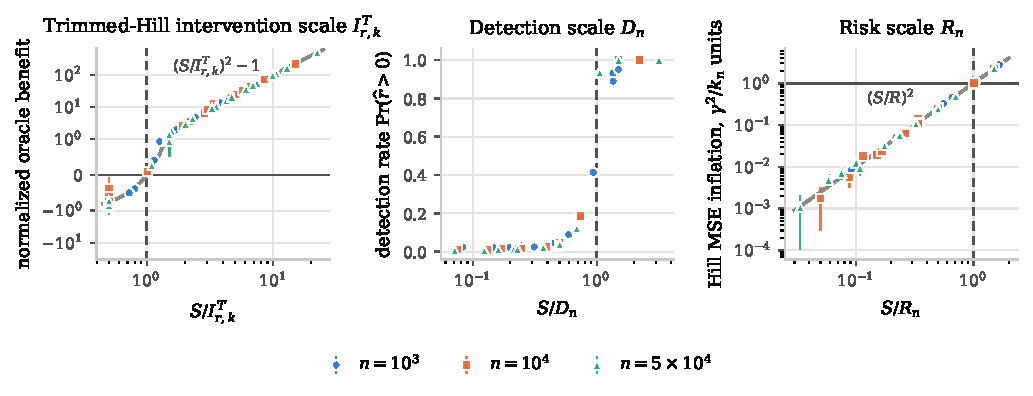
\includegraphics[width=\textwidth]{generated/fig_three_scales.pdf}
\caption{The frozen run against each of the three normalized scales.  Every
positive-signal cell of the frozen grid appears in all three panels; the dashed vertical line is that
panel's boundary and the grey curve is the exact prediction where one exists.
Error bars are Monte Carlo standard errors of the paired replicate losses in
the outer panels and Wilson $95\%$ intervals in the detection panel.  Each
panel's own boundary is the point at which its quantity changes character: the
oracle benefit changes sign at $I^{T}_{r,k}$, the scan transitions around
$D_n$, and the
Hill MSE inflation reaches the clean sampling error at $R_n$.  Tables
\ref{tab:first-run-adaptive}--\ref{tab:stress-n1000} give the underlying
numbers}
\label{fig:three-scales}
\end{figure}

\FloatBarrier

\section{Post-Specified Stress Tests}
\label{sec:stress}

The experiment of Section \ref{sec:first-run} was pre-specified, and nothing in
it is revised here.  The three studies below were specified \emph{after} those
results were seen, and are reported as post-specified throughout.  Each asks how
far the three-scale picture depends on a choice that produced it: the vanishing
family-wise level, the equal-factor contamination model, and exact Pareto
sampling.  They use a separate driver, a separate seed and separate artifacts.

\subsection{The detection transition and the level regime}

The frozen grid places signals only at $0.5D_n$ and $1.5D_n$, which establishes
a difference but does not locate a transition.  The asymptotic ordering
$I^{T}_{r,k}\ll D_n$ also depends on the vanishing level
$\alpha_n=\min\{0.05,1/\log^2n\}$: with a fixed $\alpha$ the detection scale
$D_n=\gamma\log(h_n/\alpha)$ is constant in $n$, so it is $O(1)$ like
$I^{T}_{r,k}$ and the two no longer separate asymptotically.  That is a real
restriction on the theory, and a separate question from the finite-sample
behaviour.

Table \ref{tab:stress-detection} maps detection on a grid in $S/D_n$ under both
regimes.  The transition is sharp but centred slightly below one: detection is $0.03$--$0.08$ at $0.4D_n$, has reached $0.73$--$0.86$
at $S=D_n$ itself, and is complete by $S\approx1.2D_n$.  Reporting only
$0.5D_n$ and $1.5D_n$ therefore understates how quickly the scan turns on.  And
the two level regimes give nearly the same curve once each is normalized by its
own $D_n$, the fixed-level detector being uniformly slightly more willing to
trim.  Over the sample sizes studied the two levels differ little in any case:
$D_n/\gamma$ is $5.298$ for fixed $\alpha=0.05$ against $6.743$ and $7.065$ for
the vanishing level at $n=10^4$ and $5\times10^4$, because $\log(1/\alpha_n)$
grows like $2\log\log n$.  The vanishing level is therefore not needed for the
finite-sample location of the normalized transition.  It is needed for two
other things: the asymptotic separation $I^{T}_{r,k}\ll D_n$ under this design,
and the vanishing false-rejection probability that Theorem
\ref{thm:exact-recovery} assumes.  With $\alpha$ held fixed the clean
false-trim probability does not vanish, so exact recovery is no longer the same
statement even where the detection transition sits in the same place.

\begin{table}[H]
\centering
\small
\begin{tabular}{ccccc}
\toprule
$S/D_n$ & \multicolumn{2}{c}{$n=10^4$} & \multicolumn{2}{c}{$n=5{\times}10^4$}\\
 & vanishing & fixed & vanishing & fixed\\
\midrule
$0.4$ & $0.027$ & $0.079$ & $0.023$ & $0.084$\\
$0.6$ & $0.076$ & $0.152$ & $0.065$ & $0.168$\\
$0.7$ & $0.139$ & $0.231$ & $0.129$ & $0.234$\\
$0.8$ & $0.269$ & $0.372$ & $0.241$ & $0.378$\\
$0.9$ & $0.466$ & $0.574$ & $0.493$ & $0.603$\\
$1.0$ & $0.734$ & $0.792$ & $0.810$ & $0.863$\\
$1.1$ & $0.909$ & $0.938$ & $0.974$ & $0.986$\\
$1.2$ & $0.983$ & $0.990$ & $0.999$ & $1.000$\\
$1.3$ & $0.998$ & $0.999$ & $1.000$ & $1.000$\\
$1.5$ & $1.000$ & $1.000$ & $1.000$ & $1.000$\\
$2.0$ & $1.000$ & $1.000$ & $1.000$ & $1.000$\\
\bottomrule
\end{tabular}
\caption{Post-specified detection transition at $r=5$.  Entries are $\Pp(\widehat r>0)$ on a grid in $S/D_n$, under the vanishing family-wise level $\alpha_n=\min\{0.05,1/\log^2n\}$ of the primary design and under a fixed $\alpha=0.05$.  Each column normalizes by its own $D_n$.  The transition is centred slightly below $S/D_n=1$ and is complete by $S/D_n\approx1.2$ in both regimes, so the normalized finite-sample transition is similar under fixed and vanishing levels.  The vanishing level additionally supplies the asymptotic $I^{T}_{r,k}\ll D_n$ separation and the vanishing false-rejection probability that Theorem \ref{thm:exact-recovery} assumes.}
\label{tab:stress-detection}
\end{table}


\subsection{Contamination that is not localized on one spacing}

Equal-factor contamination is exceptionally favourable to a spacing scan.  By
Lemma \ref{lem:boundary} it moves exactly one normalized spacing, so a problem
posed as $r$ contaminated extremes is really a single-spike detection problem,
and the scan is built to find exactly that spike.  Lemma \ref{lem:unequal}
already says unequal factors behave differently, but the frozen design does not
run them.

Table \ref{tab:stress-profile} does.  Taking $\log\Delta_j=c(r-j+1)$ puts
spacing shifts $jc$ on every $j\le r$ with the same total, so by Lemma
\ref{lem:unequal} the contaminated-Hill MSE is unchanged: across the cells at
$S\ge1.5D_n$ the two profiles differ in measured contamination cost by at most
$5.6\%$.  Detection is not similarly unchanged.  At $S=1.5D_n$ the
equal-factor signal is detected in every replicate, while the spread signal is
detected in as few as $2.5\%$ of them; at $n=10^4$ and $r=10$ the rates are
$1.000$ against $0.029$, and the adaptive benefit falls from
$2.39\times10^{-3}$ to $4.55\times10^{-5}$.  The degradation grows with $r$,
which is what dividing a fixed signal among more spacings should do.

The experiment says which contamination the scan misses; the reason is
algebraic.  Write $\boldsymbol\delta=(\delta_1,\ldots,\delta_r)$ for the
spacing-shift vector of Remark \ref{rem:delta}.  Contamination enters the scan
statistic of Section \ref{sec:detection-scale} through both of its arguments:
\[
  R_j^\star
  =
  \frac{Z_j+\delta_j}
       {\overline Z_{j+1:k_n}
        +\dfrac1{k_n-j}\displaystyle\sum_{\ell=j+1}^{r}\delta_\ell},
\]
since the deeper spacings that form the denominator are themselves contaminated
when $j<r$.  The numerator sees one component of $\boldsymbol\delta$; the
denominator sees the tail of the vector divided by $k_n-j$.

\begin{proposition}[Localization-controlled spacing detectability]
\label{prop:localization}
Work in the exact-Pareto model with ordered factors
$\Delta_1\ge\cdots\ge\Delta_r\ge1$, so $\boldsymbol\delta_n\ge0$.  Assume
$1\le r_n\le h_n<k_n$, $r_n=O(1)$, $\|\boldsymbol\delta_n\|_1=o(k_n)$,
$L_n=\log(h_n/\alpha_n)\to\infty$ and $L_n=o(k_n)$, and put
\[
  M_n=\|\boldsymbol\delta_n\|_\infty=\max_{1\le j\le r_n}\delta_{n,j}.
\]
Then, for every fixed $\varepsilon>0$,
\[
  \frac{M_n}{\gamma L_n}\ge1+\varepsilon
  \quad\Longrightarrow\quad
  \Pp(\hbox{some contaminated spacing is rejected})\to1,
\]
and, for every fixed $\varepsilon\in(0,1)$,
\[
  \frac{M_n}{\gamma L_n}\le1-\varepsilon
  \quad\Longrightarrow\quad
  \Pp(\hbox{any contaminated spacing is rejected})\to0.
\]
\end{proposition}

\begin{proof}
Write $D_{n,j}$ for the denominator of $R_j^\star$.  The contamination it
carries is bounded by
\[
  \frac1{k_n-j}\sum_{\ell=j+1}^{r_n}\delta_{n,\ell}
  \le
  \frac{\|\boldsymbol\delta_n\|_1}{k_n-r_n}
  =o(1),
\]
because $\|\boldsymbol\delta_n\|_1=o(k_n)$ and $r_n=O(1)$.  Since
$k_n-j\to\infty$, the law of large numbers gives
$\overline Z_{j+1:k_n}\to_p\gamma$, so $D_{n,j}\to_p\gamma$; as $r_n=O(1)$
there are boundedly many contaminated indices and the convergence is uniform
over $j\le r_n$.  The exact rejection threshold obeys $t_{m_n,a_n}/L_n\to1$ as
in Proposition \ref{prop:detectability}.  Because $r_n\le h_n$, every
contaminated spacing is among those the scan tests.

Suppose first $M_n\ge(1+\varepsilon)\gamma L_n$, and let $j^\star\le r_n$
attain $M_n$.  Under exact Pareto sampling $Z_{j^\star}\ge0$, so the numerator
of $R_{j^\star}^\star$ is at least $M_n$, and with probability tending to one
$D_{n,j^\star}\le\gamma(1+\varepsilon/4)$.  On that event
\[
  \frac{R_{j^\star}^\star}{L_n}
  \ge
  \frac{M_n}{\gamma(1+\varepsilon/4)L_n}
  \ge
  \frac{1+\varepsilon}{1+\varepsilon/4}
  >1,
\]
a bound that does not require $M_n/L_n$ to stay bounded, and the threshold ratio
tends to one, so $j^\star$ is rejected with probability tending to one.

Suppose instead $M_n\le(1-\varepsilon)\gamma L_n$.  Every
$\delta_{n,j}/L_n$ is then bounded by $(1-\varepsilon)\gamma$.  The
contamination in the denominator is nonnegative, so
$D_{n,j}\ge\overline Z_{j+1:k_n}$, which exceeds $\gamma(1-\varepsilon/2)$
with probability tending to one, and $Z_j/L_n=o_p(1)$ because $Z_j=O_p(1)$ and
$L_n\to\infty$.  Hence, uniformly over $j\le r_n$,
\[
  \frac{R_j^\star}{L_n}
  \le
  \frac{Z_j/L_n+(1-\varepsilon)\gamma}{\gamma(1-\varepsilon/2)}
  \longrightarrow_p
  \frac{1-\varepsilon}{1-\varepsilon/2}
  <1 .
\]
A union bound over the boundedly many contaminated indices gives the second
claim.
\end{proof}

The proposition concerns the contaminated spacings only.  It says nothing about
false rejections among the clean spacings, which the level $\alpha_n$ controls
separately, and it is therefore not a statement about recovering $r_n$.

Which quantity matters depends on the question.  Hill damage is aggregate: by Remark \ref{rem:delta},
$\ghat_H^\star-\ghat_H=\|\boldsymbol\delta\|_1/k_n$.  Detection of \emph{some}
contaminated spacing is local, and Proposition \ref{prop:localization} puts its
boundary at $\|\boldsymbol\delta\|_\infty\asymp\gamma L_n=D_n$.  Exact recovery
of the count is deeper still: the deepest-first scan of Theorem
\ref{thm:exact-recovery} returns $\widehat r_n=r_n$ only if the boundary
spacing itself is rejected, so the relevant component is $\delta_r$, combined
as before with the vanishing false-rejection probability that $\alpha_n\to0$
supplies.  A large $\|\boldsymbol\delta\|_\infty$ at some interior $j<r$ does
not by itself deliver exact recovery.

For a nonzero, nonnegative $\boldsymbol\delta\in\mathbb R^r$ define the
localization coefficient
\[
  \kappa(\boldsymbol\delta)
  =
  \frac{\|\boldsymbol\delta\|_\infty}{\|\boldsymbol\delta\|_1}
  \in\left[\frac1r,1\right],
\]
with $\kappa=1$ when a single spacing carries the whole shift and $\kappa=1/r$
when all $r$ carry it equally.  The equal-factor model of the primary
experiment is the extreme case: there $\boldsymbol\delta=(0,\ldots,0,S)$, so
$\kappa=1$ and $\|\boldsymbol\delta\|_1=\|\boldsymbol\delta\|_\infty=S$, which
is why one scalar sufficed.  In general, writing $S=\|\boldsymbol\delta\|_1$
for the aggregate signal, the largest local jump available to the scan is
$\kappa S$, and Proposition \ref{prop:localization} places the detection
boundary at
\[
  \kappa S\asymp D_n,
  \qquad\hbox{equivalently}\qquad
  S_{\mathrm{detect}}\asymp\frac{D_n}{\kappa}.
\]
This is a localization-adjusted reading of this particular spacing scan under
the stated sparse regime, not a detectability boundary for contamination in
general or for other detectors.

The spread profile already run is a direct test of that reading, and requires
no further simulation.  With $\log\Delta_j=c(r-j+1)$ the shifts are
$\delta_j=jc$, so $\|\boldsymbol\delta\|_1=cr(r+1)/2$ and
$\|\boldsymbol\delta\|_\infty=\delta_r=rc$, giving
\[
  \kappa=\frac2{r+1}.
\]
At the $S=2.5D_n$ cells of Table \ref{tab:stress-profile} this predicts local
jumps of $\kappa S=1.25D_n$, $0.833D_n$ and $0.455D_n$ at $r=3$, $5$ and $10$,
and the measured detection rates fall in that order: $0.994$ and $1.000$ at
$r=3$, $0.358$ and $0.372$ at $r=5$, and $0.060$ and $0.055$ at $r=10$, for
$n=10^4$ and $5\times10^4$.  The agreement is quantitative as well as ordinal.
Linear interpolation of the equal-factor detection curve of Table
\ref{tab:stress-detection} in $S/D_n$, read at $\kappa S/D_n$ instead of
$S/D_n$, predicts $0.991$, $0.335$ and $0.040$ at
$n=10^4$ against the measured $0.994$, $0.358$ and $0.060$; that curve is
itself nearly independent of $r$, agreeing to within $0.01$ between $r=1$ and
$r=5$.  The small systematic under-prediction is expected, since the spread
profile elevates several spacings at once and the scan tests each of them,
while the equal-factor curve describes a single spike of the same height.

This is the sharpest limitation of the paper.  Equally damaging contamination
is not equally detectable, so $D_n$ is a detection scale for spacing-localized
contamination rather than for contamination of a given magnitude.

The consequence for Theorem \ref{thm:detect-ignore} is stronger than a
restriction on $D_n$: the dichotomy itself does not extend.  The theorem holds
because contamination is either large enough to be recovered or small enough to
be first-order negligible, and under the equal-factor geometry those two cases
exhaust the possibilities.  Under spread contamination they do not.  Since
$D_n/R_n=0.674$ at $n=10^4$, the cell at $S=1.5D_n$ already has $S/R_n=1.011$,
so the contamination has reached the first-order Hill-risk scale; with $r=10$
its detection probability is $0.029$ and its recovery probability $0.006$.  The
same happens further out: at $S=2.5D_n$, where $S/R_n=1.686$, detection is
still only $0.060$.  Nine cells of the spread design have $S/R_n\ge1$ and four
of them are detected in under a tenth of replications.  A contamination can
therefore be simultaneously undetected and first-order relevant, which is
precisely the case Theorem \ref{thm:detect-ignore} excludes.

That does not contradict the theorem, which is stated for the equal-factor
model and proved there.  It does say that the theorem is specific to that
geometry rather than to sparse contamination generally, and that a
detect-or-ignore statement for unequal factors would need a detection scale
built from the local jumps $j\log(\Delta_j/\Delta_{j+1})$ rather than from the
total $S$.

\begin{table}[H]
\centering
\footnotesize
\setlength{\tabcolsep}{4pt}
\begin{tabular}{cccccccc}
\toprule
$n$ & $r$ & $S/D_n$ & \multicolumn{2}{c}{detection} & unit & \multicolumn{2}{c}{$\widehat B_n^{(A)}$}\\
 & & & equal & spread & & equal & spread\\
\midrule
$10^4$ & $3$ & $0.5$ & $0.043$ & $0.018$ & $10^{-5}$ & $-5.58\pm1.03$ & $-2.82\pm0.95$\\
$10^4$ & $3$ & $1.0$ & $0.723$ & $0.052$ & $10^{-5}$ & $9.39\pm4.02$ & $0.18\pm1.65$\\
$10^4$ & $3$ & $1.5$ & $1.000$ & $0.218$ & $10^{-3}$ & $2.52\pm0.07$ & $0.08\pm0.04$\\
$10^4$ & $3$ & $2.5$ & $1.000$ & $0.994$ & $10^{-3}$ & $7.00\pm0.12$ & $6.70\pm0.12$\\
$10^4$ & $5$ & $0.5$ & $0.035$ & $0.020$ & $10^{-5}$ & $-2.48\pm0.97$ & $-0.81\pm0.99$\\
$10^4$ & $5$ & $1.0$ & $0.733$ & $0.028$ & $10^{-5}$ & $0.52\pm4.13$ & $-1.20\pm1.30$\\
$10^4$ & $5$ & $1.5$ & $1.000$ & $0.065$ & $10^{-3}$ & $2.37\pm0.07$ & $0.05\pm0.02$\\
$10^4$ & $5$ & $2.5$ & $1.000$ & $0.358$ & $10^{-3}$ & $6.86\pm0.12$ & $1.07\pm0.08$\\
$10^4$ & $10$ & $0.5$ & $0.040$ & $0.016$ & $10^{-5}$ & $-2.65\pm1.19$ & $-0.21\pm0.80$\\
$10^4$ & $10$ & $1.0$ & $0.725$ & $0.021$ & $10^{-5}$ & $-1.31\pm4.37$ & $1.04\pm1.02$\\
$10^4$ & $10$ & $1.5$ & $1.000$ & $0.029$ & $10^{-3}$ & $2.39\pm0.08$ & $0.05\pm0.02$\\
$10^4$ & $10$ & $2.5$ & $1.000$ & $0.060$ & $10^{-3}$ & $6.66\pm0.12$ & $0.30\pm0.03$\\
\midrule
$5{\times}10^4$ & $3$ & $0.5$ & $0.040$ & $0.014$ & $10^{-5}$ & $-1.33\pm0.36$ & $0.11\pm0.25$\\
$5{\times}10^4$ & $3$ & $1.0$ & $0.817$ & $0.047$ & $10^{-5}$ & $2.09\pm1.33$ & $-1.47\pm0.50$\\
$5{\times}10^4$ & $3$ & $1.5$ & $1.000$ & $0.192$ & $10^{-4}$ & $5.55\pm0.23$ & $0.20\pm0.12$\\
$5{\times}10^4$ & $3$ & $2.5$ & $1.000$ & $1.000$ & $10^{-3}$ & $1.59\pm0.04$ & $1.59\pm0.04$\\
$5{\times}10^4$ & $5$ & $0.5$ & $0.035$ & $0.014$ & $10^{-6}$ & $-8.63\pm3.14$ & $-6.05\pm2.43$\\
$5{\times}10^4$ & $5$ & $1.0$ & $0.827$ & $0.025$ & $10^{-5}$ & $2.09\pm1.39$ & $-0.62\pm0.34$\\
$5{\times}10^4$ & $5$ & $1.5$ & $1.000$ & $0.052$ & $10^{-4}$ & $5.30\pm0.23$ & $0.16\pm0.07$\\
$5{\times}10^4$ & $5$ & $2.5$ & $1.000$ & $0.372$ & $10^{-3}$ & $1.54\pm0.04$ & $0.23\pm0.02$\\
$5{\times}10^4$ & $10$ & $0.5$ & $0.040$ & $0.013$ & $10^{-6}$ & $-7.35\pm3.00$ & $-2.21\pm1.82$\\
$5{\times}10^4$ & $10$ & $1.0$ & $0.808$ & $0.016$ & $10^{-5}$ & $-0.54\pm1.44$ & $-0.18\pm0.28$\\
$5{\times}10^4$ & $10$ & $1.5$ & $1.000$ & $0.025$ & $10^{-4}$ & $5.05\pm0.24$ & $0.10\pm0.05$\\
$5{\times}10^4$ & $10$ & $2.5$ & $1.000$ & $0.055$ & $10^{-3}$ & $1.50\pm0.04$ & $0.07\pm0.01$\\
\bottomrule
\end{tabular}
\caption{Post-specified comparison of contamination profiles at matched Hill bias.  The equal-factor profile places the whole signal on spacing $r$; the spread profile uses unequal factors chosen so that, by Lemma \ref{lem:unequal}, the shifts $jc$ fall on all of $j=1,\ldots,r$ and the total, hence the contaminated-Hill MSE, is unchanged.  The two profiles damage Hill identically but are not equally detectable: at $S=1.5D_n$ the equal-factor signal is detected in every replicate while the spread signal is detected in a few percent of them, and the adaptive benefit falls with it.  $D_n$ is therefore a detection scale for spacing-localized contamination, not for contamination of a given magnitude.}
\label{tab:stress-profile}
\end{table}


\FloatBarrier

\subsection{Second-order tails}

Under exact Pareto sampling the normalized spacings are exactly iid
exponential, which is what makes two of the three scales exact identities.
Pareto-type tails admit only an approximate exponential representation
\citep{beirlant-dierckx-guillou-starica-2002}, and ordinary Hill then carries
threshold bias.  Table \ref{tab:stress-second-order} samples the Burr law
\[
  \overline F(x)=(1+x^{c})^{-\lambda},
  \qquad
  \gamma=\frac1{c\lambda},
  \qquad
  \rho=-\frac1\lambda,
\]
so that $\gamma=1/2$ with $\rho\in\{-1,-1/2,-1/4\}$ at
$(\lambda,c)=(1,2),(2,1),(4,1/2)$.  The top $k_n+1$ order statistics are
generated exactly from uniform order statistics rather than by drawing the full
sample; feeding the same generator the exact-Pareto survival quantile returns
spacings with mean $0.4992$ and variance $0.2496$ against the targets
$\gamma=0.5$ and $\gamma^2=0.25$, which validates the construction.

The two exact identities of Section \ref{sec:first-run} cannot survive this
change.  Lemma \ref{lem:boundary} is a deterministic identity between
spacings, so $\ghat_H^\star=\ghat_H+S/k_n$
whatever law the spacings follow, and therefore
\[
  \operatorname{MSE}(\ghat_H^\star)-\operatorname{MSE}(\ghat_H)
  =
  \frac{S^2}{k_n^2}
  +
  \frac{2S}{k_n}\,\E(\ghat_H-\gamma).
\]
The second term vanishes only when Hill is unbiased, which is exactly what
exact Pareto sampling guarantees.  Under a second-order tail it is proportional
to the threshold bias, and at $\rho=-1/4$ it is the larger of the two terms.
What is tested below is therefore the detection organization, not the risk
identities.

Detection stays near its clean level at $0.5D_n$ and is essentially complete
at $1.5D_n$ for every $\rho$, falling only to $0.907$ in the most biased cell,
and above $D_n$ adaptive trimming approaches the trim-count oracle as recovery
becomes nearly complete.  What survives is therefore the detection
organization; what changes is the risk decomposition, because threshold bias
contributes materially to the Hill MSE.  At $\rho=-0.25$ and $n=10^4$
the contaminated-Hill MSE at $1.5D_n$ is $5.4\times10^{-2}$ while the
contamination contributes $2.0\times10^{-2}$ of it; the rest is threshold bias.
In that regime the contamination question is secondary to the choice of $k_n$,
which the exact-Pareto model removes by construction.

\begin{table}[H]
\centering
\footnotesize
\setlength{\tabcolsep}{4pt}
\begin{tabular}{cccccccc}
\toprule
$n$ & $\rho$ & $S/D_n$ & $\operatorname{MSE}(\ghat_H^\star)$ & detection & unit & adaptive & oracle\\
\midrule
$10^4$ & $-1.00$ & $0.0$ & $2.60{\times}10^{-3}$ & $0.013$ & $10^{-4}$ & $-0.11\pm0.07$ & $-1.30\pm0.17$\\
$10^4$ & $-1.00$ & $0.5$ & $2.92{\times}10^{-3}$ & $0.040$ & $10^{-4}$ & $-0.16\pm0.11$ & $3.17\pm0.28$\\
$10^4$ & $-1.00$ & $1.5$ & $5.23{\times}10^{-3}$ & $1.000$ & $10^{-3}$ & $2.60\pm0.07$ & $2.60\pm0.07$\\
$10^4$ & $-0.50$ & $0.0$ & $4.01{\times}10^{-3}$ & $0.008$ & $10^{-4}$ & $0.13\pm0.06$ & $-2.74\pm0.23$\\
$10^4$ & $-0.50$ & $0.5$ & $5.57{\times}10^{-3}$ & $0.029$ & $10^{-3}$ & $0.03\pm0.01$ & $1.24\pm0.03$\\
$10^4$ & $-0.50$ & $1.5$ & $1.04{\times}10^{-2}$ & $0.999$ & $10^{-3}$ & $5.95\pm0.08$ & $5.95\pm0.08$\\
$10^4$ & $-0.25$ & $0.0$ & $3.37{\times}10^{-2}$ & $0.003$ & $10^{-3}$ & $0.03\pm0.01$ & $-2.13\pm0.07$\\
$10^4$ & $-0.25$ & $0.5$ & $3.98{\times}10^{-2}$ & $0.011$ & $10^{-3}$ & $0.17\pm0.03$ & $3.95\pm0.07$\\
$10^4$ & $-0.25$ & $1.5$ & $5.44{\times}10^{-2}$ & $0.907$ & $10^{-2}$ & $1.58\pm0.01$ & $1.79\pm0.01$\\
\midrule
$5{\times}10^4$ & $-1.00$ & $0.0$ & $1.12{\times}10^{-3}$ & $0.010$ & $10^{-5}$ & $-0.10\pm0.20$ & $-1.16\pm0.50$\\
$5{\times}10^4$ & $-1.00$ & $0.5$ & $1.21{\times}10^{-3}$ & $0.039$ & $10^{-5}$ & $-0.77\pm0.33$ & $4.12\pm0.91$\\
$5{\times}10^4$ & $-1.00$ & $1.5$ & $1.69{\times}10^{-3}$ & $1.000$ & $10^{-4}$ & $5.83\pm0.23$ & $5.83\pm0.23$\\
$5{\times}10^4$ & $-0.50$ & $0.0$ & $1.81{\times}10^{-3}$ & $0.006$ & $10^{-5}$ & $0.25\pm0.12$ & $-4.15\pm0.63$\\
$5{\times}10^4$ & $-0.50$ & $0.5$ & $2.27{\times}10^{-3}$ & $0.031$ & $10^{-4}$ & $0.22\pm0.04$ & $3.95\pm0.10$\\
$5{\times}10^4$ & $-0.50$ & $1.5$ & $3.40{\times}10^{-3}$ & $1.000$ & $10^{-3}$ & $1.61\pm0.02$ & $1.61\pm0.02$\\
$5{\times}10^4$ & $-0.25$ & $0.0$ & $1.91{\times}10^{-2}$ & $0.004$ & $10^{-4}$ & $0.14\pm0.04$ & $-6.17\pm0.22$\\
$5{\times}10^4$ & $-0.25$ & $0.5$ & $2.15{\times}10^{-2}$ & $0.008$ & $10^{-3}$ & $0.04\pm0.01$ & $1.54\pm0.02$\\
$5{\times}10^4$ & $-0.25$ & $1.5$ & $2.58{\times}10^{-2}$ & $1.000$ & $10^{-3}$ & $6.24\pm0.03$ & $6.23\pm0.03$\\
\bottomrule
\end{tabular}
\caption{Post-specified second-order stress test at $r=5$, sampling a Burr law with second-order parameter $\rho$ rather than exact Pareto, so the normalized spacings are only approximately exponential and ordinary Hill carries threshold bias.  The detection transition survives: detection stays near its clean level at $0.5D_n$ and is essentially complete at $1.5D_n$ for every $\rho$, and above $D_n$ adaptive trimming approaches the trim-count oracle as recovery becomes nearly complete.  What changes is the relative importance of the contamination: at $\rho=-0.25$ the bias term dominates $\operatorname{MSE}(\ghat_H^\star)$, so the contamination question is secondary to threshold choice.}
\label{tab:stress-second-order}
\end{table}


\FloatBarrier

\subsection{What the stress tests change}

The stress tests produce two robustness results and one substantive
limitation.  First, $D_n$ continues to organize the transition under fixed and
vanishing family-wise levels.  Second, the detection organization persists in
the Burr experiments considered here --- signals at $0.5D_n$ stay near the
clean detection rate, signals at $1.5D_n$ are almost always found, and adaptive
trimming approaches the trim-count oracle once recovery is nearly complete ---
while the exact-Pareto risk identities do not carry over, because threshold
bias then contributes materially to the Hill MSE.  By contrast, $D_n$ does not
characterize detectability for contamination distributed across several
spacings.  It governs contamination that concentrates on one spacing, and
equally
damaging contamination spread over several spacings can be nearly invisible to
the scan even after it reaches the first-order risk scale.  That bounds the
reach of Theorem \ref{thm:detect-ignore} as well as of $D_n$, and Section
\ref{sec:discussion} treats it as the main open direction rather than as a
defect in the separation the paper is about.

\FloatBarrier

\section{Discussion}
\label{sec:discussion}

\paragraph{Three scales, not one.}
A single contamination signal $S_n=r_n\log\Delta_n$ enters three different
decisions through three different normalizations, and the frozen experiment
separates them.  Trim-count-oracle removal changes the sign of its MSE benefit
at $I^{T}_{r,k}$, the conservative spacing scan transitions around $D_n$, and
ordinary
Hill risk is disturbed at first order at $R_n$.  Two of the three are exact
identities in the exact-Pareto model and the run reproduces both: the Hill MSE
inflation matches $(S/R_n)^2$ with median observed-to-predicted ratios $1.006$,
$0.978$ and $0.999$ across the three sample sizes, and the normalized oracle
benefit matches $(S/I^{T}_{r,k})^2-1$ with median residuals $0.017$, $-0.071$
and $-0.034$.  The detection transition has no closed form and is reported as
measured; it is the sharpest of the three.

\paragraph{Within the equal-factor regime, exact recovery is not the decision
objective.}
The detect-or-ignore result of Theorem \ref{thm:detect-ignore} says that the
two ways of failing to recover the contamination are not equally costly, and
the primary experiment shows both halves.  Within that geometry, above $D_n$
the scan recovers the boundary and adaptive trimming inherits the oracle's
benefit.  Below $D_n$ it usually does not, but the contamination it misses is
then small on the first-order risk scale: among the frozen grid points at
$n\ge10^4$, the largest signal left undetected in more than half of
replications has $S/R_n=0.5$.  An estimator can therefore miss contamination
without that miss mattering at the scale on which ordinary Hill error is
measured.  Recovery is a diagnostic target; risk is the decision target, and
the two come apart in the band the three scales delimit.  Outside the
equal-factor geometry the second half of that statement fails, as Section
\ref{sec:stress} shows: spread contamination can stay undetected past
$S/R_n=1$.

\paragraph{What bounded influence adds.}
The region where bounded influence can matter is $I^{T}_{r,k}<S<D_n$, where
removal is already worthwhile but the conservative scan cannot reliably find
what to remove.  There the harmonic-moment estimators limit the contamination's
effect without identifying the contaminated boundary, and Table
\ref{tab:estimator-crossover} shows that at $n=10^4$ the $\beta=0.5$ member has
a positive benefit in cells where adaptive trimming has a negative one.  The
effect is real but not uniform: at $n=5\times10^4$ the same comparison is
within Monte Carlo error, and Tables \ref{tab:beta-r-sweep} and
\ref{tab:beta-full-contrasts} show that the advantage belongs to particular
members rather than to bounded influence as a class.  Averaged
over the frozen grid at $n\ge10^4$, $\beta=0.5$ beats adaptive trimming in
$20$ of $47$ cells, $\beta=1$ in $5$, and $\beta=2$ in none.

\paragraph{Why no robust method dominates.}
Each philosophy pays for its protection in a different currency.  Trimming pays
variance for the spacings it discards, which is why the oracle itself is
harmful below $I^{T}_{r,k}$ and why adaptive trimming is slightly harmful below
$D_n$, where it trims only by mistake.  Bounded influence pays a standing
efficiency cost that it incurs whether or not contamination is present, which
is why every harmonic-moment member is behind adaptive trimming both in the
clean control of Table \ref{tab:clean-cell}, where its cost is an order of
magnitude larger than the adaptive estimator's, and in the $0.5I$ cells.  Increasing $\beta$ bounds influence
more aggressively but carries a larger clean-sample efficiency cost, so the
family is itself a trade-off rather than a ranking.  No member is best
everywhere, and the location at which adaptive
trimming overtakes a given member depends on $\beta$, $r$ and $n$ rather than
coinciding with $D_n$.

\paragraph{Two quantities, not one.}
Proposition \ref{prop:localization} replaces the single signal $S$ by two
coordinates of the shift vector, and the four regions they define explain why
Theorem \ref{thm:detect-ignore} does not extend beyond the equal-factor model.
Writing $x=\|\boldsymbol\delta\|_\infty/D_n$ for local detectability and
$y=\|\boldsymbol\delta\|_1/R_n$ for first-order Hill relevance,
\[
\begin{array}{l|cc}
\toprule
 & y\lesssim1 & y\gtrsim1\\
\midrule
x\lesssim1 & \hbox{undetected, negligible}
           & \hbox{\bf undetected, first-order relevant}\\
x\gtrsim1 & \hbox{detected, negligible}
          & \hbox{detected, first-order relevant}\\
\bottomrule
\end{array}
\]
Under equal factors $\kappa=1$, so $x$ and $y$ are the same signal measured
against $D_n$ and $R_n$; with $D_n\ll R_n$ the top-right cell is then empty,
which is what makes the detect-or-ignore dichotomy available.  Once
$\kappa<1$ the two coordinates separate by the factor $\kappa$, and the
spread-contamination cells of Section \ref{sec:stress} sit in that cell: at
$n=10^4$, $r=10$ and $S=1.5D_n$ the aggregate signal has $y=1.011$ while the
largest local jump has $x=2/11\times1.5=0.27$.  In words, $\ell^1$ controls
Hill damage and $\ell^\infty$ controls local detectability; exact count
recovery additionally needs the deepest jump $\delta_r$ to clear $D_n$.  This
describes the spacing scan studied here under the stated sparse regime, not
every possible detector.

\paragraph{Limitations.}
The model is deliberately narrow.  Sampling is exact Pareto, so there is no
second-order bias term and no bias-variance trade-off in the choice of $k_n$;
the three scales are therefore clean, but real threshold selection is not.  The
contamination is applied to the top $r_n$ order statistics after their ranks
are known and with a common factor, which is a structural stress test rather
than Huber contamination.  Lemma \ref{lem:unequal} shows that unequal factors
decouple the detection signal from the Hill bias, and Section
\ref{sec:stress} measures the size of that decoupling: contamination spread
over several spacings can damage Hill identically and still be nearly
invisible to the scan, and can stay so after reaching the first-order risk
scale.  That limits Theorem \ref{thm:detect-ignore} as well as $D_n$: outside
the equal-factor geometry, detection and negligibility no longer exhaust the
possibilities, so extending the detect-or-ignore statement to unequal factors
is the paper's main open problem rather than a routine generalization.  The experiment fixes $\gamma=0.5$
because all three scales are proportional to $\gamma$, uses the single
threshold rate $k_n=\lfloor n^{1/2}\rfloor$, and holds $r$ in $\{1,3,5,10\}$, so
regimes with $r_n\to\infty$ are untested.  It is one frozen run of 5000
replications from one seed; the Monte Carlo standard errors reported throughout
quantify that, and the $n=10^3$ row shows how far the asymptotic ordering can
be from a finite sample.

\paragraph{Relation to the robust tail-estimation literature.}
The contribution is a separation of decision questions rather than a new
estimator, so it sits alongside rather than against the trim-and-detect and
bounded-influence lines.  Robust Pareto estimation has been compared on bias
and RMSE across many estimators and contamination schemes
\citep{brzezinski-2016}, and the efficiency price of protection is long
established \citep{brazauskas-serfling-2000,finkelstein-tucker-veeh-2006}; the
clean control here reproduces that price rather than avoiding it.  What the
three scales add is an answer to a prior question: when the price is worth
paying, when the contamination can be found at all, and when it matters to
first-order risk.  Among spacing-based work, Hsieh \citeyearpar{hsieh-1999} and
Minkah, de Wet and Ghosh \citeyearpar{minkah-dewet-ghosh-2023} act on the same
statistics used here, deciding how much tail to use and how to downweight
spacings respectively, rather than how many contaminated order statistics to
remove.

\paragraph{Open problems.}
The following extend the results without being prerequisites for them.
\begin{enumerate}
\item Extend Proposition \ref{prop:localization} into a full unequal-factor
detect-or-ignore result, characterizing when local detectability
$\|\boldsymbol\delta_n\|_\infty$ and aggregate relevance
$\|\boldsymbol\delta_n\|_1$ together permit or preclude first-order
robustness.
\item Extend Theorem \ref{thm:detect-ignore} to contamination counts with
$r_n\to\infty$ but $r_n=o(k_n)$, identifying the growth rates for which finite
trimming remains first-order negligible.
\item Convert the harmonic-moment mean-shift calculation into a full MSE
comparison with Hill, oracle trimming and adaptive trimming.  Section
\ref{sec:first-run} gives that comparison empirically; what is still missing is
the analytic counterpart, and in particular a characterization of the risk
crossover that Tables \ref{tab:estimator-crossover} and
\ref{tab:beta-contrasts} place somewhat above the detection boundary.
\item Compare fixed trimming, adaptive trimming and bounded-influence
estimators under the same sparse contamination sequence, extending the finite
grid of Section \ref{sec:first-run} to a sequence in $n$.
\item Characterize the intervention scale for oracles outside the trimmed-Hill
family, following Remark \ref{rem:trim-oracle}: under the equal-factor model a
procedure that knew which single spacing was shifted could act on less
information loss than $r$-trimming requires.
\end{enumerate}

\section{Conclusion}

Robust tail-index estimation is often judged by whether a method finds the
contaminated extremes.  In the exact-Pareto model studied here, that criterion
answers a different question from the one a user of the estimator faces.  A
sparse multiplicative contamination of the top $r_n$ order statistics enters
through one scalar $S_n=r_n\log\Delta_n$, and that scalar has to be compared
with three separate scales before anything follows.  None of the three is a
scale of the contamination alone: each belongs to a procedure.  For standard
$r$-trimmed Hill, $I^{T}_{r,k}$ decides whether removal repays its variance
cost; for the conservative spacing scan at level $\alpha_n$ with $h_n$
candidate boundaries, $D_n$ decides whether the contamination can be found at
all; and for ordinary Hill under squared error, $R_n$ decides whether the
contamination matters at the scale on which its error is measured.  For bounded contamination counts $r_n$ these scales are ordered
$I^{T}_{r,k}\ll D_n\ll R_n$, so the intermediate regions are not empty.  A
pre-specified Monte Carlo experiment reproduces the two exact risk identities
at finite $n$ and exhibits the predicted detection transition around $D_n$.

The practical consequence, within the equal-factor regime of Theorem
\ref{thm:detect-ignore}, is that adaptive trimming may safely fail to recover
weak contamination, and that below $I^{T}_{r,k}$ intervention within the
standard trimmed-Hill family is not MSE-beneficial, because its variance cost
then exceeds the contamination bias it removes.  Outside that geometry the two
come apart: for ordered unequal factors, $\|\boldsymbol\delta\|_1$ controls
Hill's contamination shift while $\|\boldsymbol\delta\|_\infty$ controls this
spacing scan's local detectability, so contamination can be damaging and
undetectable at once.  The detection scale determines
when reliable removal becomes feasible.  The risk comparison between removal and bounding influence
depends additionally on the efficiency cost of the bounded-influence procedure,
and therefore on $\beta$, $r$ and $n$, rather than on which estimator is more
robust in the abstract.  Detection,
worthwhile intervention, and first-order risk relevance are different
statistical questions.

\section*{Statements and Declarations}

\paragraph{Funding.}
No funding was received for conducting this study.

\paragraph{Competing interests.}
The author has no relevant financial or non-financial interests to disclose.

\section*{Data and Code Availability}

The study uses no empirical data.  All results come from the simulations
described in Sections \ref{sec:frozen-design}, \ref{sec:first-run} and
\ref{sec:stress}.  The complete replication package --- the simulation drivers,
the analysis-only scripts, the frozen summary and per-replicate losses, the
configuration and provenance records, this manuscript with its generated table
and figure fragments, and a SHA-256 manifest covering every file --- is
archived at Zenodo under \texttt{10.5281/zenodo.22171166}.  Online Resource~1
supplies a compact reproduction guide containing that manifest, the
configuration and provenance summary, a map from each table and figure to the
file that produces it, and the archive's identifier.  Reproducing every number
reported here requires only the analysis scripts and the frozen artifacts, not
a re-run of the simulation.

The estimators and the spacing scan are those of the \texttt{heavytails}
package version $0.5.0$, archived at
\url{https://doi.org/10.5281/zenodo.22070996} \citep{heavytails-2026}.  Both
identifiers belong to the same repository but to different releases: 0.5.0 is
the software that produced the results, while the replication archive named
above is release 0.6.2, the first to contain the package.

\appendix

\section{Pre-Asymptotic Stress Test at \texorpdfstring{$n=10^3$}{n = 1000}}
\label{app:stress}

The frozen design includes $n=10^3$ explicitly as a pre-asymptotic stress test,
because at that sample size $D_n>R_n$ and the intended ordering of the three
scales fails.  Section \ref{sec:first-run} therefore restricts its detection and
estimator comparisons to the two larger sample sizes, where the ordering holds.
The clean control of Table \ref{tab:clean-cell} and the intervention check of
Table \ref{tab:intervention} do include $n=10^3$, because neither depends on
how $D_n$ and $R_n$ are ordered.  The rest of the pre-specified row is reported
here rather than dropped.

Table \ref{tab:stress-n1000} shows what breaks down, and it is not the theory.
With $k_n=\lfloor n^{1/2}\rfloor=31$, the intervention scale
$I^{T}_{r,k}=\gamma\{rk_n/(k_n-r)\}^{1/2}$ grows quickly in $r$, and at $r=10$ it
exceeds the detection and risk grid points themselves: the $0.5D$ cell has
$S/I^{T}_{r,k}=0.803$ and the $0.5R$ cell has $S/I^{T}_{r,k}=0.725$.  Those cells carry
labels defined as fractions of $D_n$ and $R_n$ but in fact lie below
$I^{T}_{r,k}$, so at $n=10^3$ the frozen signal grid no longer brackets the three
scales in the intended order.  The clearly negative oracle benefits there
are exactly what Proposition \ref{prop:oracle-intervention} predicts below the
intervention scale.  Across the whole frozen run, at all three sample sizes,
every clearly negative oracle benefit occurs in a cell with $S<I^{T}_{r,k}$.

The detection behavior degrades in the same way and for the same reason.  At
$1.5D$ detection is $0.951$--$0.988$ rather than $1.0000$, and the clean-control
no-trim rate falls to $0.9768$ $[0.9746,0.9787]$.  Both are consequences of
$k_n=31$: the scan has few spacings to work with and the level
$\alpha_n=\min\{0.05,1/\log^2n\}$ is at its least conservative here.  Nothing in
this row contradicts the asymptotic statements; it shows the sample size at
which the design's own scale separation has not yet appeared.

\begin{table}[t]
\centering
\small
\begin{tabular}{cccccccc}
\toprule
$S$ & $r$ & $S/I^{T}_{r,k}$ & $S/D_n$ & $S/R_n$ & detection $[95\%]$ & $\widehat B_n^{(A)}$ & $\widehat B_n^{(T)}$\\
\midrule
$0.5I$ & $1$ & $0.500$ & $0.082$ & $0.091$ & $0.0238$ $[0.0199,0.0284]$ & $(-2.51\pm0.44)10^{-4}$ & $(-2.43\pm0.47)10^{-4}$\\
$0.5I$ & $3$ & $0.500$ & $0.148$ & $0.164$ & $0.0196$ $[0.0161,0.0238]$ & $(-2.45\pm0.48)10^{-4}$ & $(-6.90\pm0.86)10^{-4}$\\
$0.5I$ & $5$ & $0.500$ & $0.198$ & $0.219$ & $0.0226$ $[0.0188,0.0271]$ & $(-1.41\pm0.41)10^{-4}$ & $(-1.11\pm0.11)10^{-3}$\\
$0.5I$ & $10$ & $0.500$ & $0.311$ & $0.345$ & $0.0246$ $[0.0207,0.0293]$ & $(-1.91\pm0.55)10^{-4}$ & $(-2.88\pm0.19)10^{-3}$\\
$1.5I$ & $1$ & $1.500$ & $0.247$ & $0.274$ & $0.0298$ $[0.0254,0.0349]$ & $(-2.41\pm0.58)10^{-4}$ & $(2.93\pm0.73)10^{-4}$\\
$1.5I$ & $3$ & $1.500$ & $0.443$ & $0.491$ & $0.0476$ $[0.0420,0.0539]$ & $(-3.46\pm0.68)10^{-4}$ & $(1.06\pm0.13)10^{-3}$\\
$1.5I$ & $5$ & $1.500$ & $0.594$ & $0.658$ & $0.0896$ $[0.0820,0.0978]$ & $(-6.51\pm0.86)10^{-4}$ & $(2.11\pm0.18)10^{-3}$\\
$1.5I$ & $10$ & $1.500$ & $0.934$ & $1.035$ & $0.4134$ $[0.3998,0.4271]$ & $(-1.82\pm0.19)10^{-3}$ & $(4.71\pm0.28)10^{-3}$\\
$0.5D$ & $1$ & $3.034$ & $0.500$ & $0.554$ & $0.0658$ $[0.0593,0.0730]$ & $(-5.63\pm0.75)10^{-4}$ & $(2.27\pm0.14)10^{-3}$\\
$0.5D$ & $3$ & $1.692$ & $0.500$ & $0.554$ & $0.0670$ $[0.0604,0.0743]$ & $(-5.41\pm0.85)10^{-4}$ & $(1.69\pm0.14)10^{-3}$\\
$0.5D$ & $5$ & $1.263$ & $0.500$ & $0.554$ & $0.0568$ $[0.0507,0.0636]$ & $(-4.24\pm0.75)10^{-4}$ & $(1.45\pm0.17)10^{-3}$\\
$0.5D$ & $10$ & $0.803$ & $0.500$ & $0.554$ & $0.0558$ $[0.0498,0.0625]$ & $(-5.33\pm0.81)10^{-4}$ & $(-1.51\pm0.22)10^{-3}$\\
$1.5D$ & $1$ & $9.101$ & $1.500$ & $1.662$ & $0.9878$ $[0.9844,0.9905]$ & $(2.09\pm0.04)10^{-2}$ & $(2.20\pm0.04)10^{-2}$\\
$1.5D$ & $3$ & $5.076$ & $1.500$ & $1.662$ & $0.9812$ $[0.9770,0.9846]$ & $(1.96\pm0.04)10^{-2}$ & $(2.10\pm0.04)10^{-2}$\\
$1.5D$ & $5$ & $3.789$ & $1.500$ & $1.662$ & $0.9758$ $[0.9712,0.9797]$ & $(1.94\pm0.04)10^{-2}$ & $(2.09\pm0.04)10^{-2}$\\
$1.5D$ & $10$ & $2.408$ & $1.500$ & $1.662$ & $0.9506$ $[0.9442,0.9563]$ & $(1.66\pm0.04)10^{-2}$ & $(1.85\pm0.04)10^{-2}$\\
$0.5R$ & $1$ & $2.739$ & $0.451$ & $0.500$ & $0.0504$ $[0.0447,0.0568]$ & $(-3.73\pm0.66)10^{-4}$ & $(1.58\pm0.12)10^{-3}$\\
$0.5R$ & $3$ & $1.528$ & $0.451$ & $0.500$ & $0.0468$ $[0.0413,0.0530]$ & $(-3.41\pm0.64)10^{-4}$ & $(1.29\pm0.13)10^{-3}$\\
$0.5R$ & $5$ & $1.140$ & $0.451$ & $0.500$ & $0.0506$ $[0.0449,0.0570]$ & $(-3.55\pm0.78)10^{-4}$ & $(6.42\pm1.57)10^{-4}$\\
$0.5R$ & $10$ & $0.725$ & $0.451$ & $0.500$ & $0.0442$ $[0.0388,0.0503]$ & $(-4.65\pm0.75)10^{-4}$ & $(-1.93\pm0.20)10^{-3}$\\
$1.5R$ & $1$ & $8.216$ & $1.354$ & $1.500$ & $0.9468$ $[0.9402,0.9527]$ & $(1.48\pm0.03)10^{-2}$ & $(1.81\pm0.03)10^{-2}$\\
$1.5R$ & $3$ & $4.583$ & $1.354$ & $1.500$ & $0.9422$ $[0.9354,0.9483]$ & $(1.41\pm0.03)10^{-2}$ & $(1.74\pm0.04)10^{-2}$\\
$1.5R$ & $5$ & $3.421$ & $1.354$ & $1.500$ & $0.9302$ $[0.9228,0.9369]$ & $(1.29\pm0.03)10^{-2}$ & $(1.61\pm0.03)10^{-2}$\\
$1.5R$ & $10$ & $2.174$ & $1.354$ & $1.500$ & $0.8890$ $[0.8800,0.8974]$ & $(1.09\pm0.03)10^{-2}$ & $(1.43\pm0.04)10^{-2}$\\
\bottomrule
\end{tabular}
\caption{Pre-asymptotic stress test at $n=10^3$, the pre-specified row where $D_n>R_n$ and the intended ordering of the scales does not hold.  Detection is $\Pp(\widehat r>0)$ with a Wilson $95\%$ interval; $\widehat B_n^{(A)}$ and $\widehat B_n^{(T)}$ are the paired adaptive and oracle benefits against contaminated Hill.  The $S/I^{T}_{r,k}$ column shows why this row is a stress test: with $k_n=31$ and $r=10$ the intervention scale exceeds the detection and risk grid points ($S/I^{T}_{r,k}=0.80$ at $0.5D$ and $0.72$ at $0.5R$), so the frozen signal grid no longer brackets the three scales in the intended order. The clearly negative oracle benefits in those cells are what Proposition \ref{prop:oracle-intervention} predicts below $I^{T}_{r,k}$, not a failure of the oracle.}
\label{tab:stress-n1000}
\end{table}


\begin{table}[t]
\centering
\small
\begin{tabular}{cccccc}
\toprule
$n$ & $S$ & $r$ cells & $\beta{=}0.5$ & $\beta{=}1$ & $\beta{=}2$\\
\midrule
$10^3$ & $0.5I$ & $4$ & $0$ & $0$ & $0$\\
$10^3$ & $1.5I$ & $4$ & $4$ & $3$ & $2$\\
$10^3$ & $0.5D$ & $4$ & $3$ & $3$ & $0$\\
$10^3$ & $1.5D$ & $4$ & $0$ & $0$ & $0$\\
$10^3$ & $0.5R$ & $4$ & $3$ & $3$ & $0$\\
$10^3$ & $1.5R$ & $4$ & $1$ & $2$ & $2$\\
\midrule
$10^4$ & $0.5I$ & $4$ & $0$ & $0$ & $0$\\
$10^4$ & $1.5I$ & $3$ & $2$ & $0$ & $0$\\
$10^4$ & $1.5I{=}0.5R$ & $1$ & $1$ & $1$ & $0$\\
$10^4$ & $0.5D$ & $4$ & $4$ & $0$ & $0$\\
$10^4$ & $1.5D$ & $4$ & $0$ & $0$ & $0$\\
$10^4$ & $0.5R$ & $3$ & $3$ & $3$ & $0$\\
$10^4$ & $1.5R$ & $4$ & $0$ & $0$ & $0$\\
\midrule
$5{\times}10^4$ & $0.5I$ & $4$ & $0$ & $0$ & $0$\\
$5{\times}10^4$ & $1.5I$ & $4$ & $2$ & $1$ & $0$\\
$5{\times}10^4$ & $0.5D$ & $4$ & $4$ & $0$ & $0$\\
$5{\times}10^4$ & $1.5D$ & $4$ & $0$ & $0$ & $0$\\
$5{\times}10^4$ & $0.5R$ & $4$ & $4$ & $0$ & $0$\\
$5{\times}10^4$ & $1.5R$ & $4$ & $0$ & $0$ & $0$\\
\bottomrule
\end{tabular}
\caption{Bounded influence against adaptive trimming across the whole frozen grid.  For each design point, the last three columns count the contamination counts $r\in\{1,3,5,10\}$ at which that harmonic-moment member has the larger paired benefit against contaminated Hill.  This is the evidence behind the family-level statements of Section \ref{sec:first-run}, which Tables \ref{tab:estimator-crossover} and \ref{tab:beta-contrasts} report at $r=5$ only.  At $n\ge10^4$ the most aggressively bounded member, $\beta=2$, never beats adaptive trimming; the four cells where it does are all in the pre-asymptotic $n=10^3$ row.}
\label{tab:beta-r-sweep}
\end{table}


\begin{table}[t]
\centering
\footnotesize
\begin{tabular}{ccccccc}
\toprule
$n$ & $S$ & $r$ & $S/D_n$ & $\beta{=}0.5$ & $\beta{=}1$ & $\beta{=}2$\\
\midrule
$10^4$ & $0.5I$ & $1$ & $0.075$ & $-5.9$ & $-11.0$ & $-16.9$\\
$10^4$ & $0.5I$ & $3$ & $0.130$ & $-5.5$ & $-11.3$ & $-18.7$\\
$10^4$ & $0.5I$ & $5$ & $0.170$ & $-6.2$ & $-12.1$ & $-18.9$\\
$10^4$ & $0.5I$ & $10$ & $0.247$ & $-3.4$ & $-9.0$ & $-16.5$\\
$10^4$ & $1.5I$ & $1$ & $0.224$ & $-4.0$ & $-10.8$ & $-18.3$\\
$10^4$ & $1.5I$ & $3$ & $0.391$ & $1.0$ & $-6.4$ & $-15.4$\\
$10^4$ & $1.5I$ & $5$ & $0.510$ & $6.1$ & $-2.0$ & $-12.7$\\
$10^4$ & $0.5D$ & $1$ & $0.500$ & $9.2$ & $-0.3$ & $-11.9$\\
$10^4$ & $0.5D$ & $3$ & $0.500$ & $8.2$ & $-0.1$ & $-10.9$\\
$10^4$ & $0.5D$ & $5$ & $0.500$ & $6.7$ & $-1.2$ & $-11.9$\\
$10^4$ & $0.5D$ & $10$ & $0.500$ & $4.3$ & $-1.7$ & $-11.2$\\
$10^4$ & $1.5D$ & $1$ & $1.500$ & $-5.2$ & $-10.5$ & $-17.4$\\
$10^4$ & $1.5D$ & $3$ & $1.500$ & $-10.7$ & $-10.1$ & $-17.9$\\
$10^4$ & $1.5D$ & $5$ & $1.500$ & $-13.4$ & $-9.3$ & $-16.2$\\
$10^4$ & $1.5D$ & $10$ & $1.500$ & $-16.9$ & $-10.4$ & $-13.6$\\
$10^4$ & $0.5R$ & $1$ & $0.741$ & $22.0$ & $10.0$ & $-3.9$\\
$10^4$ & $0.5R$ & $3$ & $0.741$ & $21.3$ & $10.8$ & $-3.4$\\
$10^4$ & $0.5R$ & $5$ & $0.741$ & $19.4$ & $10.2$ & $-3.6$\\
$10^4$ & $1.5R$ & $1$ & $2.224$ & $-6.3$ & $-11.3$ & $-17.9$\\
$10^4$ & $1.5R$ & $3$ & $2.224$ & $-14.5$ & $-9.9$ & $-17.3$\\
$10^4$ & $1.5R$ & $5$ & $2.224$ & $-20.3$ & $-11.5$ & $-16.6$\\
$10^4$ & $1.5R$ & $10$ & $2.224$ & $-27.1$ & $-15.1$ & $-14.8$\\
\midrule
$5{\times}10^4$ & $0.5I$ & $1$ & $0.071$ & $-7.6$ & $-12.5$ & $-18.7$\\
$5{\times}10^4$ & $0.5I$ & $3$ & $0.123$ & $-5.9$ & $-11.5$ & $-18.8$\\
$5{\times}10^4$ & $0.5I$ & $5$ & $0.160$ & $-6.8$ & $-12.4$ & $-19.4$\\
$5{\times}10^4$ & $0.5I$ & $10$ & $0.229$ & $-5.9$ & $-11.3$ & $-18.1$\\
$5{\times}10^4$ & $1.5I$ & $1$ & $0.213$ & $-4.0$ & $-10.3$ & $-18.1$\\
$5{\times}10^4$ & $1.5I$ & $3$ & $0.370$ & $-1.8$ & $-8.4$ & $-16.5$\\
$5{\times}10^4$ & $1.5I$ & $5$ & $0.480$ & $0.3$ & $-6.4$ & $-14.9$\\
$5{\times}10^4$ & $1.5I$ & $10$ & $0.687$ & $8.8$ & $1.4$ & $-8.8$\\
$5{\times}10^4$ & $0.5D$ & $1$ & $0.500$ & $2.1$ & $-5.9$ & $-15.4$\\
$5{\times}10^4$ & $0.5D$ & $3$ & $0.500$ & $1.4$ & $-6.3$ & $-15.6$\\
$5{\times}10^4$ & $0.5D$ & $5$ & $0.500$ & $1.6$ & $-5.7$ & $-14.8$\\
$5{\times}10^4$ & $0.5D$ & $10$ & $0.500$ & $0.2$ & $-6.5$ & $-15.4$\\
$5{\times}10^4$ & $1.5D$ & $1$ & $1.500$ & $-7.8$ & $-13.2$ & $-19.6$\\
$5{\times}10^4$ & $1.5D$ & $3$ & $1.500$ & $-7.7$ & $-10.9$ & $-17.7$\\
$5{\times}10^4$ & $1.5D$ & $5$ & $1.500$ & $-8.9$ & $-11.2$ & $-19.0$\\
$5{\times}10^4$ & $1.5D$ & $10$ & $1.500$ & $-9.4$ & $-9.3$ & $-16.9$\\
$5{\times}10^4$ & $0.5R$ & $1$ & $1.057$ & $5.0$ & $-4.4$ & $-15.0$\\
$5{\times}10^4$ & $0.5R$ & $3$ & $1.057$ & $6.3$ & $-1.2$ & $-12.0$\\
$5{\times}10^4$ & $0.5R$ & $5$ & $1.057$ & $4.8$ & $-1.6$ & $-12.8$\\
$5{\times}10^4$ & $0.5R$ & $10$ & $1.057$ & $3.4$ & $-0.1$ & $-10.9$\\
$5{\times}10^4$ & $1.5R$ & $1$ & $3.170$ & $-7.4$ & $-12.6$ & $-19.0$\\
$5{\times}10^4$ & $1.5R$ & $3$ & $3.170$ & $-8.3$ & $-10.3$ & $-17.9$\\
$5{\times}10^4$ & $1.5R$ & $5$ & $3.170$ & $-14.5$ & $-10.6$ & $-17.7$\\
$5{\times}10^4$ & $1.5R$ & $10$ & $3.170$ & $-22.2$ & $-12.7$ & $-17.5$\\
\bottomrule
\end{tabular}
\caption{Paired contrasts of every frozen bounded-influence member against adaptive trimming, at every contamination count of the grid.  Entries are paired $t$ statistics for the replicate loss differences $d_i=(\ghat_{A,i}^\star-\gamma)^2-(\ghat_{\beta,i}^\star-\gamma)^2$, so $t>0$ favours bounded influence.  Table \ref{tab:beta-contrasts} is the $r=5$ block of this table and Table \ref{tab:beta-r-sweep} its sign pattern; the magnitudes are given here so that the family-level statements of Section \ref{sec:first-run} can be checked cell by cell.}
\label{tab:beta-full-contrasts}
\end{table}


\FloatBarrier

\begin{thebibliography}{99}

\bibitem[Beirlant et al.(2002)]{beirlant-dierckx-guillou-starica-2002}
J. Beirlant, G. Dierckx, A. Guillou, and C. St\u{a}ric\u{a}.
\newblock On exponential representations of log-spacings of extreme order
statistics.
\newblock \emph{Extremes}, 5(2):157--180, 2002.
\newblock \url{https://doi.org/10.1023/A:1022171205129}

\bibitem[Beran and Schell(2012)]{beran-schell-2012}
J. Beran and D. Schell.
\newblock On robust tail index estimation.
\newblock \emph{Computational Statistics \& Data Analysis}, 56(11):3430--3443,
2012.
\newblock \url{https://doi.org/10.1016/j.csda.2010.05.028}

\bibitem[Beran et al.(2014)]{beran-schell-stehlik-2014}
J. Beran, D. Schell, and M. Stehlik.
\newblock The harmonic moment tail index estimator: asymptotic distribution
and robustness.
\newblock \emph{Annals of the Institute of Statistical Mathematics},
66(1):193--220, 2014.
\newblock \url{https://doi.org/10.1007/s10463-013-0412-2}

\bibitem[Bhattacharya et al.(2019)]{bhattacharya-kallitsis-stoev-2019}
S. Bhattacharya, M. Kallitsis, and S. Stoev.
\newblock Data-adaptive trimming of the Hill estimator and detection of
outliers in the extremes of heavy-tailed data.
\newblock \emph{Electronic Journal of Statistics}, 13(1):1872--1925, 2019.
\newblock \url{https://doi.org/10.1214/19-EJS1561}

\bibitem[Brazauskas and Serfling(2000)]{brazauskas-serfling-2000}
V. Brazauskas and R. Serfling.
\newblock Robust and efficient estimation of the tail index of a
single-parameter Pareto distribution.
\newblock \emph{North American Actuarial Journal}, 4(4):12--27, 2000.
\newblock \url{https://doi.org/10.1080/10920277.2000.10595935}

\bibitem[Brazauskas and Serfling(2001)]{brazauskas-serfling-2001}
V. Brazauskas and R. Serfling.
\newblock Small sample performance of robust estimators of tail parameters for
Pareto and exponential models.
\newblock \emph{Journal of Statistical Computation and Simulation},
70(1):1--19, 2001.
\newblock \url{https://doi.org/10.1080/00949650108812103}

\bibitem[Brzezinski(2016)]{brzezinski-2016}
M. Brzezinski.
\newblock Robust estimation of the Pareto tail index: a Monte Carlo analysis.
\newblock \emph{Empirical Economics}, 51:1--30, 2016.
\newblock \url{https://doi.org/10.1007/s00181-015-0989-9}

\bibitem[de Haan and Ferreira(2006)]{dehaan-ferreira-2006}
L. de Haan and A. Ferreira.
\newblock \emph{Extreme Value Theory: An Introduction}.
\newblock Springer, New York, 2006.
\newblock \url{https://doi.org/10.1007/0-387-34471-3}

\bibitem[de Haan and Stadtmuller(1996)]{dehaan-stadtmuller-1996}
L. de Haan and U. Stadtmuller.
\newblock Generalized regular variation of second order.
\newblock \emph{Journal of the Australian Mathematical Society}, 61:381--395,
1996.
\newblock \url{https://doi.org/10.1017/S144678870000046X}

\bibitem[Dupuis and Victoria-Feser(2006)]{dupuis-victoria-feser-2006}
D. J. Dupuis and M.-P. Victoria-Feser.
\newblock A robust prediction error criterion for Pareto modelling of upper
tails.
\newblock \emph{The Canadian Journal of Statistics}, 34(4):639--658, 2006.
\newblock \url{https://doi.org/10.1002/cjs.5550340406}

\bibitem[Finkelstein et al.(2006)]{finkelstein-tucker-veeh-2006}
M. Finkelstein, H. G. Tucker, and J. A. Veeh.
\newblock Pareto tail index estimation revisited.
\newblock \emph{North American Actuarial Journal}, 10(1):1--10, 2006.
\newblock \url{https://doi.org/10.1080/10920277.2006.10596236}

\bibitem[Hill(1975)]{hill-1975}
B. M. Hill.
\newblock A simple general approach to inference about the tail of a
distribution.
\newblock \emph{The Annals of Statistics}, 3(5):1163--1174, 1975.
\newblock \url{https://doi.org/10.1214/aos/1176343247}

\bibitem[Hsieh(1999)]{hsieh-1999}
P.-H. Hsieh.
\newblock Robustness of tail index estimation.
\newblock \emph{Journal of Computational and Graphical Statistics},
8(2):318--332, 1999.
\newblock \url{https://doi.org/10.1080/10618600.1999.10474816}

\bibitem[Jordanova et al.(2016)]{jordanova-fabian-hermann-2016}
P. Jordanova, Z. Fabian, P. Hermann, et al.
\newblock Weak properties and robustness of t-Hill estimators.
\newblock \emph{Extremes}, 19:591--626, 2016.
\newblock \url{https://doi.org/10.1007/s10687-016-0256-2}

\bibitem[Minkah et al.(2023)]{minkah-dewet-ghosh-2023}
R. Minkah, T. de Wet, and A. Ghosh.
\newblock Robust estimation of Pareto-type tail index through an exponential
regression model.
\newblock \emph{Communications in Statistics --- Theory and Methods},
52(2):479--498, 2023.
\newblock \url{https://doi.org/10.1080/03610926.2021.1916530}

\bibitem[Renyi(1953)]{renyi-1953}
A. Renyi.
\newblock On the theory of order statistics.
\newblock \emph{Acta Mathematica Academiae Scientiarum Hungaricae}, 4:191--231,
1953.
\newblock \url{https://doi.org/10.1007/BF02127580}

\bibitem[Ribeiro(2026)]{heavytails-2026}
D. Ribeiro.
\newblock heavytails: a Python library for heavy-tailed probability
distributions, version 0.5.0.
\newblock Version DOI, resolving to the release used here rather than to the
most recent one.
\newblock Zenodo, 2026.
\newblock \url{https://doi.org/10.5281/zenodo.22070996}

\bibitem[Ruckdeschel and Horbenko(2013)]{ruckdeschel-horbenko-2010}
P. Ruckdeschel and N. Horbenko.
\newblock Robust estimators in generalized Pareto models.
\newblock \emph{Statistics}, 47(4):762--791, 2013.
\newblock \url{https://doi.org/10.1080/02331888.2011.628022}

\bibitem[Vandewalle et al.(2007)]{vandewalle-beirlant-christmann-hubert-2007}
B. Vandewalle, J. Beirlant, A. Christmann, and M. Hubert.
\newblock A robust estimator for the tail index of Pareto-type distributions.
\newblock \emph{Computational Statistics \& Data Analysis}, 51:6252--6268,
2007.
\newblock \url{https://doi.org/10.1016/j.csda.2007.01.003}

\end{thebibliography}

\end{document}
